\documentclass[]{bytedance_seed}

% single-column: \documentclass[]{bytedance_seed}, 
%Please prioritize using single-column。

% twocolumn: \documentclass[twocolumn]{bytedance_seed}

\usepackage[toc,page,header]{appendix}


%%%%%%%%%%%%%%%%%%%%%%%%%%%%%%%%%%%%

\usepackage{minitoc}








%%%%%%%%%%%%%%%%%%%%

\title{Reinforcing Chain-of-Thought Reasoning with Self-Evolving Rubrics}

\author[1,2,*,\ddagger]{Leheng~Sheng}
\author[1,*,\dagger]{Wenchang~Ma}
\author[1]{Ruixin~Hong} 
\author[3]{\linebreak[4] Xiang~Wang}
\author[3,\dagger]{An~Zhang}
% \author[1,\dagger]{Ke~Shen}
\author[2]{Tat-Seng~Chua}

\affiliation[1]{Seed, ByteDance}
\affiliation[2]{National University of Singapore}
\affiliation[3]{University~of~Science~and~Technology~of~China}

\contribution[*]{Equal Contribution}
\contribution[\ddagger]{Work done at ByteDance Seed}
\contribution[\dagger]{Corresponding authors}

\abstract{
Despite chain-of-thought (CoT) playing crucial roles in LLM reasoning, directly rewarding it is difficult: training a reward model demands heavy human labeling efforts, and static RMs struggle with evolving CoT distributions and reward hacking.
These challenges motivate us to seek an autonomous CoT rewarding approach that requires no human annotation efforts and can evolve gradually. 
Inspired by recent self-evolving training methods, we propose \textbf{RLCER} (\textbf{R}einforcement \textbf{L}earning with \textbf{C}oT Supervision via Self-\textbf{E}volving \textbf{R}ubrics), which enhances the outcome-centric RLVR by rewarding CoTs with self-proposed and self-evolving rubrics. 
We show that self-proposed and self-evolving rubrics provide reliable CoT supervision signals even without outcome rewards, enabling RLCER to outperform outcome-centric RLVR.
Moreover, when used as in-prompt hints, these self-proposed rubrics further improve inference-time performance.
}

\date{\today}

% \correspondence{
% An Zhang at \email{an\_zhang@ustc.edu.cn},
% Ke Shen at \email{shenke@bytedance.com}
% }

\correspondence{
An Zhang at \email{an\_zhang@ustc.edu.cn}
Wenchang Ma at \email{mawenchang.99@bytedance.com}
}


% You can add additional info fields as follows 
\checkdata[Project Page]{\url{https://alphalab-ustc.github.io/rlcer-alphalab/}}

% New packages
\usepackage{amsmath}
\usepackage{amssymb}
\usepackage{mathtools}
\usepackage{amsthm}
\usepackage{soul}
\usepackage{wrapfig}

%%%%%%%%%%%%%%%%%%%%%%%%%%%%%%%%
% THEOREMS
%%%%%%%%%%%%%%%%%%%%%%%%%%%%%%%%
\theoremstyle{plain}
\newtheorem{theorem}{Theorem}[section]
\newtheorem{proposition}[theorem]{Proposition}
\newtheorem{lemma}[theorem]{Lemma}
\newtheorem{corollary}[theorem]{Corollary}
\theoremstyle{definition}
\newtheorem{definition}[theorem]{Definition}
\newtheorem{assumption}[theorem]{Assumption}
\theoremstyle{remark}
\newtheorem{remark}[theorem]{Remark}

% Todonotes is useful during development; simply uncomment the next line
%    and comment out the line below the next line to turn off comments
%\usepackage[disable,textsize=tiny]{todonotes}
\usepackage[textsize=tiny]{todonotes}


\usepackage{enumitem}
\usepackage[table]{xcolor}  % 推荐这个，更通用
\usepackage{amsthm}     % 通常已经有
\usepackage{thmtools}   % 这个才提供 \declaretheorem
\usepackage{tcolorbox}
\usepackage{tabularx}
\usepackage{multirow} 
\usepackage{dblfloatfix}


\usepackage{tikz}
\usetikzlibrary{calc,tikzmark,backgrounds}

% 1) Define a background layer for algorithm highlighting
\pgfdeclarelayer{algobg}
\pgfsetlayers{algobg,main}

% 2) Marks used inside algorithmic
\newcommand{\tikzmk}[1]{%
  \tikz[remember picture,overlay]\node[inner sep=0pt,outer sep=0pt] (#1) {};%
}

% 3) Tunable geometry parameters (defaults)
\newlength{\algoboxshiftx}
\newlength{\algoboxpadxL}
\newlength{\algoboxpadxR}
\newlength{\algoboxpadyT}
\newlength{\algoboxpadyB}

% Default values (tweak if needed)
\setlength{\algoboxshiftx}{-0.6em}
\setlength{\algoboxpadxL}{0.6em}
\setlength{\algoboxpadxR}{-1.2em}
\setlength{\algoboxpadyT}{1.7ex}
\setlength{\algoboxpadyB}{0.8ex}

% 4) Three different background colors
% \definecolor{RolloutBg}{HTML}{2F6FEB} % base (blue-ish)
% {234,208,228}
\definecolor{RolloutBg}{RGB}{234, 208, 228}
\definecolor{RewardBg}{RGB}{250, 235, 206}
\definecolor{PolicyBg}{RGB}{217, 215, 219}

% \definecolor{RewardBg}{HTML}{FB8C00}  % base (green-ish)
% \definecolor{PolicyBg}{HTML}{FB8C00}  % base (orange-ish)

% If you prefer pastel fill directly, you can also define pastel colors instead:
% \definecolor{RolloutBg}{RGB}{232,241,255}
% \definecolor{RewardBg}{RGB}{233,248,238}
% \definecolor{PolicyBg}{RGB}{255,241,230}

% 5) boxit macro (your version; #2 is a COLOR NAME now)
% \boxit[右下角标签]{颜色}{起点mark}{终点mark}
\newcommand{\boxit}[4][]{%
\begin{tikzpicture}[remember picture,overlay]
\begin{pgfonlayer}{algobg}
  \coordinate (ALG@NW) at ([xshift=\algoboxshiftx-\algoboxpadxL,yshift=\algoboxpadyT]#3);

  \coordinate (ALG@SE) at ([xshift=\algoboxshiftx+\dimexpr\linewidth+\algoboxpadxR\relax,
                            yshift=-\algoboxpadyB]#3 |- #4);

  % fill with opacity; rounded corners
  \fill[#2, opacity=0.14, rounded corners=2pt] (ALG@NW) rectangle (ALG@SE);

  % bottom-right label (optional)
  \if\relax\detokenize{#1}\relax\else
    \node[anchor=south east, font=\scriptsize\bfseries, text=black!70]
      at ([xshift=-0.2em,yshift=0.2ex]ALG@SE) {#1};
  \fi
\end{pgfonlayer}
\end{tikzpicture}%
}

\newcommand{\ie}{\emph{i.e., }}
\newcommand{\eg}{\emph{e.g., }}
\newcommand{\etal}{\emph{et al.}}
% \newcommand{\st}{\emph{s.t. }}
\newcommand{\etc}{\emph{etc.}}
\newcommand{\wrt}{\emph{w.r.t.}~}
\newcommand{\cf}{\emph{cf. }}
\newcommand{\aka}{\emph{aka. }}

% \newcommand{\wx}[1]{{\color{black}{#1}}}
% \newcommand{\wxx}[1]{{\color{blue}{#1}}}
% \newcommand{\za}[1]{{\color{black}{#1}}}
% \newcommand{\czb}[1]{{\color{black}{#1}}}
% \newcommand{\slh}[1]{{\color{orange}{#1}}}
% \newcommand{\scs}[1]{{\color{purple}{#1}}}
% \newcommand{\cmr}[1]{{\color{black}{#1}}}
% \newcommand{\szy}[1]{{\color{black}{#1}}}
% \newcommand{\warning}[1]{{\color{red}{#1}}}
% \newcommand{\draft}[1]{{\color{black}{#1}}}
% \newcommand{\refusalv}[1]{{\color{gray}{#1}}}
% \newcommand{\concept}[1]{{\color{green}{#1}}}
% \newcommand{\revision}[1]{{\color{blue}{#1}}}
% \newcommand{\possible}[1]{{\color{black}{#1}}}

\newcommand{\wx}[1]{{\color{black}{#1}}}
\newcommand{\wxx}[1]{{\color{blue}{#1}}}
\newcommand{\za}[1]{{\color{black}{#1}}}
\newcommand{\czb}[1]{{\color{black}{#1}}}
\newcommand{\slh}[1]{{\color{black}{#1}}}
\newcommand{\scs}[1]{{\color{black}{#1}}}
\newcommand{\cmr}[1]{{\color{black}{#1}}}
\newcommand{\szy}[1]{{\color{black}{#1}}}
\newcommand{\warning}[1]{{\color{black}{#1}}}
\newcommand{\draft}[1]{{\color{black}{#1}}}
\newcommand{\refusalv}[1]{{\color{black}{#1}}}
\newcommand{\concept}[1]{{\color{black}{#1}}}
\newcommand{\revision}[1]{{\color{black}{#1}}}
\newcommand{\possible}[1]{{\color{black}{#1}}}


\definecolor{lightgray}{gray}{0.95}  % 数值越大越浅
% \definecolor{table_color}{RGB}{239,246,251}
\definecolor{table_color}{RGB}{252, 223, 208}
\declaretheorem[name=Theorem,numberwithin=section]{thm}

\newcommand{\yes}[1]{{\color{teal}{#1}}}
\newcommand{\no}[1]{{\color{red}{#1}}}



\DeclareMathOperator*{\argmax}{arg\,max}
\DeclareMathOperator*{\argmin}{arg\,min}

\DeclareMathOperator{\sign}{sign}
\DeclareMathOperator{\Tr}{Tr}
\let\ab\allowbreak


\newcommand\norm[1]{\left\lVert#1\right\rVert}
\newcommand{\Lapl}{\mathbf{\mathop{\mathcal{L}}}}
\newcommand{\lapl}{\mathcal{L}}
\newcommand{\Trans}[1]{{#1}^{\top}}
\newcommand{\Trace}[1]{tr\left({#1}\right)}
\newcommand{\Bracs}[1]{\left({#1}\right)}
\newcommand{\Mat}[1]{\mathbf{#1}}
\newcommand{\MatS}[3]{\mathbf{#1}^{#2}_{#3}}
\newcommand{\Space}[1]{\mathbb{#1}}
\newcommand{\Set}[1]{\mathcal{#1}}
\newcommand{\vectornorm}[1]{\left|\left|#1\right|\right|}
\newcommand{\bpi}{\boldsymbol{\pi}}
\newcommand{\BlockMat}[2]{\left[\begin{matrix}#1\\#2\end{matrix}\right]}
\newcommand{\BlockMatSquare}[4]{\left[\begin{matrix}#1 & #2\\#3 & #4\end{matrix}\right]}
\newcommand{\ParaTitle}[1]{\noindent\textbf{#1}}
\newcommand\myeq{\mathrel{\stackrel{\makebox[0pt]{\mbox{\normalfont\tiny def}}}{=}}}
\newcommand\eqc{\mathrel{\overset{\makebox[0pt]{\mbox{\normalfont\tiny\sffamily c}}}{=}}}


% \newcommand{\CommentBelow}[1]{%
%   \STATE{\color{gray}\footnotesize //#1}
% }
% Safe comment line for algorithmic (no list, no \item)
\usepackage{algorithm}
\usepackage{algorithmic}

% \newcommand{\CommentBelow}[1]{%
%   \STATE {\color{gray}\footnotesize // #1}%
% }

\newcommand{\CommentBelow}[1]{%
  {\color{gray}\footnotesize // #1}%
}
\newcommand{\Cmt}[1]{\hfill{\color{gray}\footnotesize // #1}}
\newcommand{\BREAK}{\STATE \textbf{break}}

% Define Box
% \definecolor{good}{RGB}{0,128,0}
% \definecolor{good}{RGB}{60,140,60}
% \definecolor{good}{RGB}{66,127,117}
\definecolor{good}{RGB}{58,113,104}
\definecolor{bad}{RGB}{180,0,0}
\definecolor{malboxborder}{RGB}{180,0,0}
\definecolor{benboxborder}{RGB}{81,91,131}
\definecolor{malboxbg}{RGB}{255,250,250}
% \definecolor{malboxbg}{RGB}{255,253,252}
% \definecolor{benboxbg}{RGB}{248,250,254}
\definecolor{benboxbg}{RGB}{251,252,254}
% \definecolor{titlebg}{RGB}{200,200,200}
\definecolor{titlebg}{RGB}{77,77,77}
\definecolor{rubricator}{RGB}{220, 105, 123}
\definecolor{reasoner}{RGB}{22, 78, 164}

\definecolor{performance_color}{RGB}{255, 248, 249}
% \definecolor{latency_color}{RGB}{242, 253, 255} 
% 上面是青色
\definecolor{latency_color}{RGB}{246, 249, 254}

% 
\newsavebox{\CaseStudy}
\newsavebox{\CaseStudyApdxOne}
\newsavebox{\CaseStudyApdxTwo}
\newsavebox{\CaseStudyApdxThree}
\newsavebox{\DSRPrompt}
\newsavebox{\CRPrompt}
\newsavebox{\GPTPrompt}

\newtcolorbox{gptpromptbox}[1][]{%
  colback=white,
  colframe=black,
  boxrule=1pt,
  arc=2pt,
  width=\textwidth,
  boxsep=2pt,
  left=2pt,
  right=2pt,
  top=2pt,
  bottom=2pt,
  title={PROMPT:}, % Title with colon
  fonttitle=\large\bfseries, % Larger and bold font
  coltitle=white, % Title text color
  colbacktitle=titlebg, % Gray background for the title
  % Remove attached title style (not supported in old versions)
  #1
}

\newtcolorbox{promptbox}[1][]{%
  colback=white,
  colframe=black,
  boxrule=1pt,
  sharp corners,
  width=\textwidth,
  % arc=2pt,
  % boxsep=5pt,
  % left=5pt,
  % right=5pt,
  % top=5pt,
  % bottom=5pt,
  boxsep=2pt,
  left=2pt,
  right=2pt,
  top=2pt,
  bottom=2pt,
  #1
}


\begin{document}
\maketitle

%不需要目录就注释掉 注意目录不要和第一页放在一块 要有\newpage
%\newpage
%\tableofcontents
%\newpage


% \begin{abstract}
Chain-of-thought (CoT) plays a crucial role in LLM reasoning, yet outcome-centric reinforcement learning with verifiable rewards (RLVR) typically optimizes only final-answer correctness, leaving CoTs largely unrewarded and potentially inducing sub-optimal reasoning strategies. 
While important, directly rewarding CoT is challenging mainly for two practical reasons: training a reward model (RM) for CoT rewarding typically requires substantial human efforts, and a static RM may fail to align with the dynamic CoT distribution changes during training and also be vulnerable to reward hacking. 
These challenges motivate us to seek an autonomous CoT rewarding approach that requires no human annotation efforts and can evolve gradually. 
Inspired by recent self-evolving training methods, we propose \textbf{RLCER} (\textbf{R}einforcement \textbf{L}earning with \textbf{C}oT Supervision via Self-\textbf{E}volving \textbf{R}ubrics), which enhances the outcome-centric RLVR by rewarding CoTs with self-proposed and self-evolving rubrics.
We show that these self-proposed and self-evolving rubrics provide meaningful CoT supervision even without outcome rewards, and RLCER outperforms the vanilla outcome-centric RLVR across datasets and LLM backbones. 
Additionally, we demonstrate that the generated rubrics can also explicitly guide better reasoning, since using them as in-prompt hints further improves the LLM reasoning performance at inference time. 
\end{abstract}


\begin{figure}[!h]
    \centering
    \begin{subfigure}[t]{0.605\columnwidth}
        \centering
        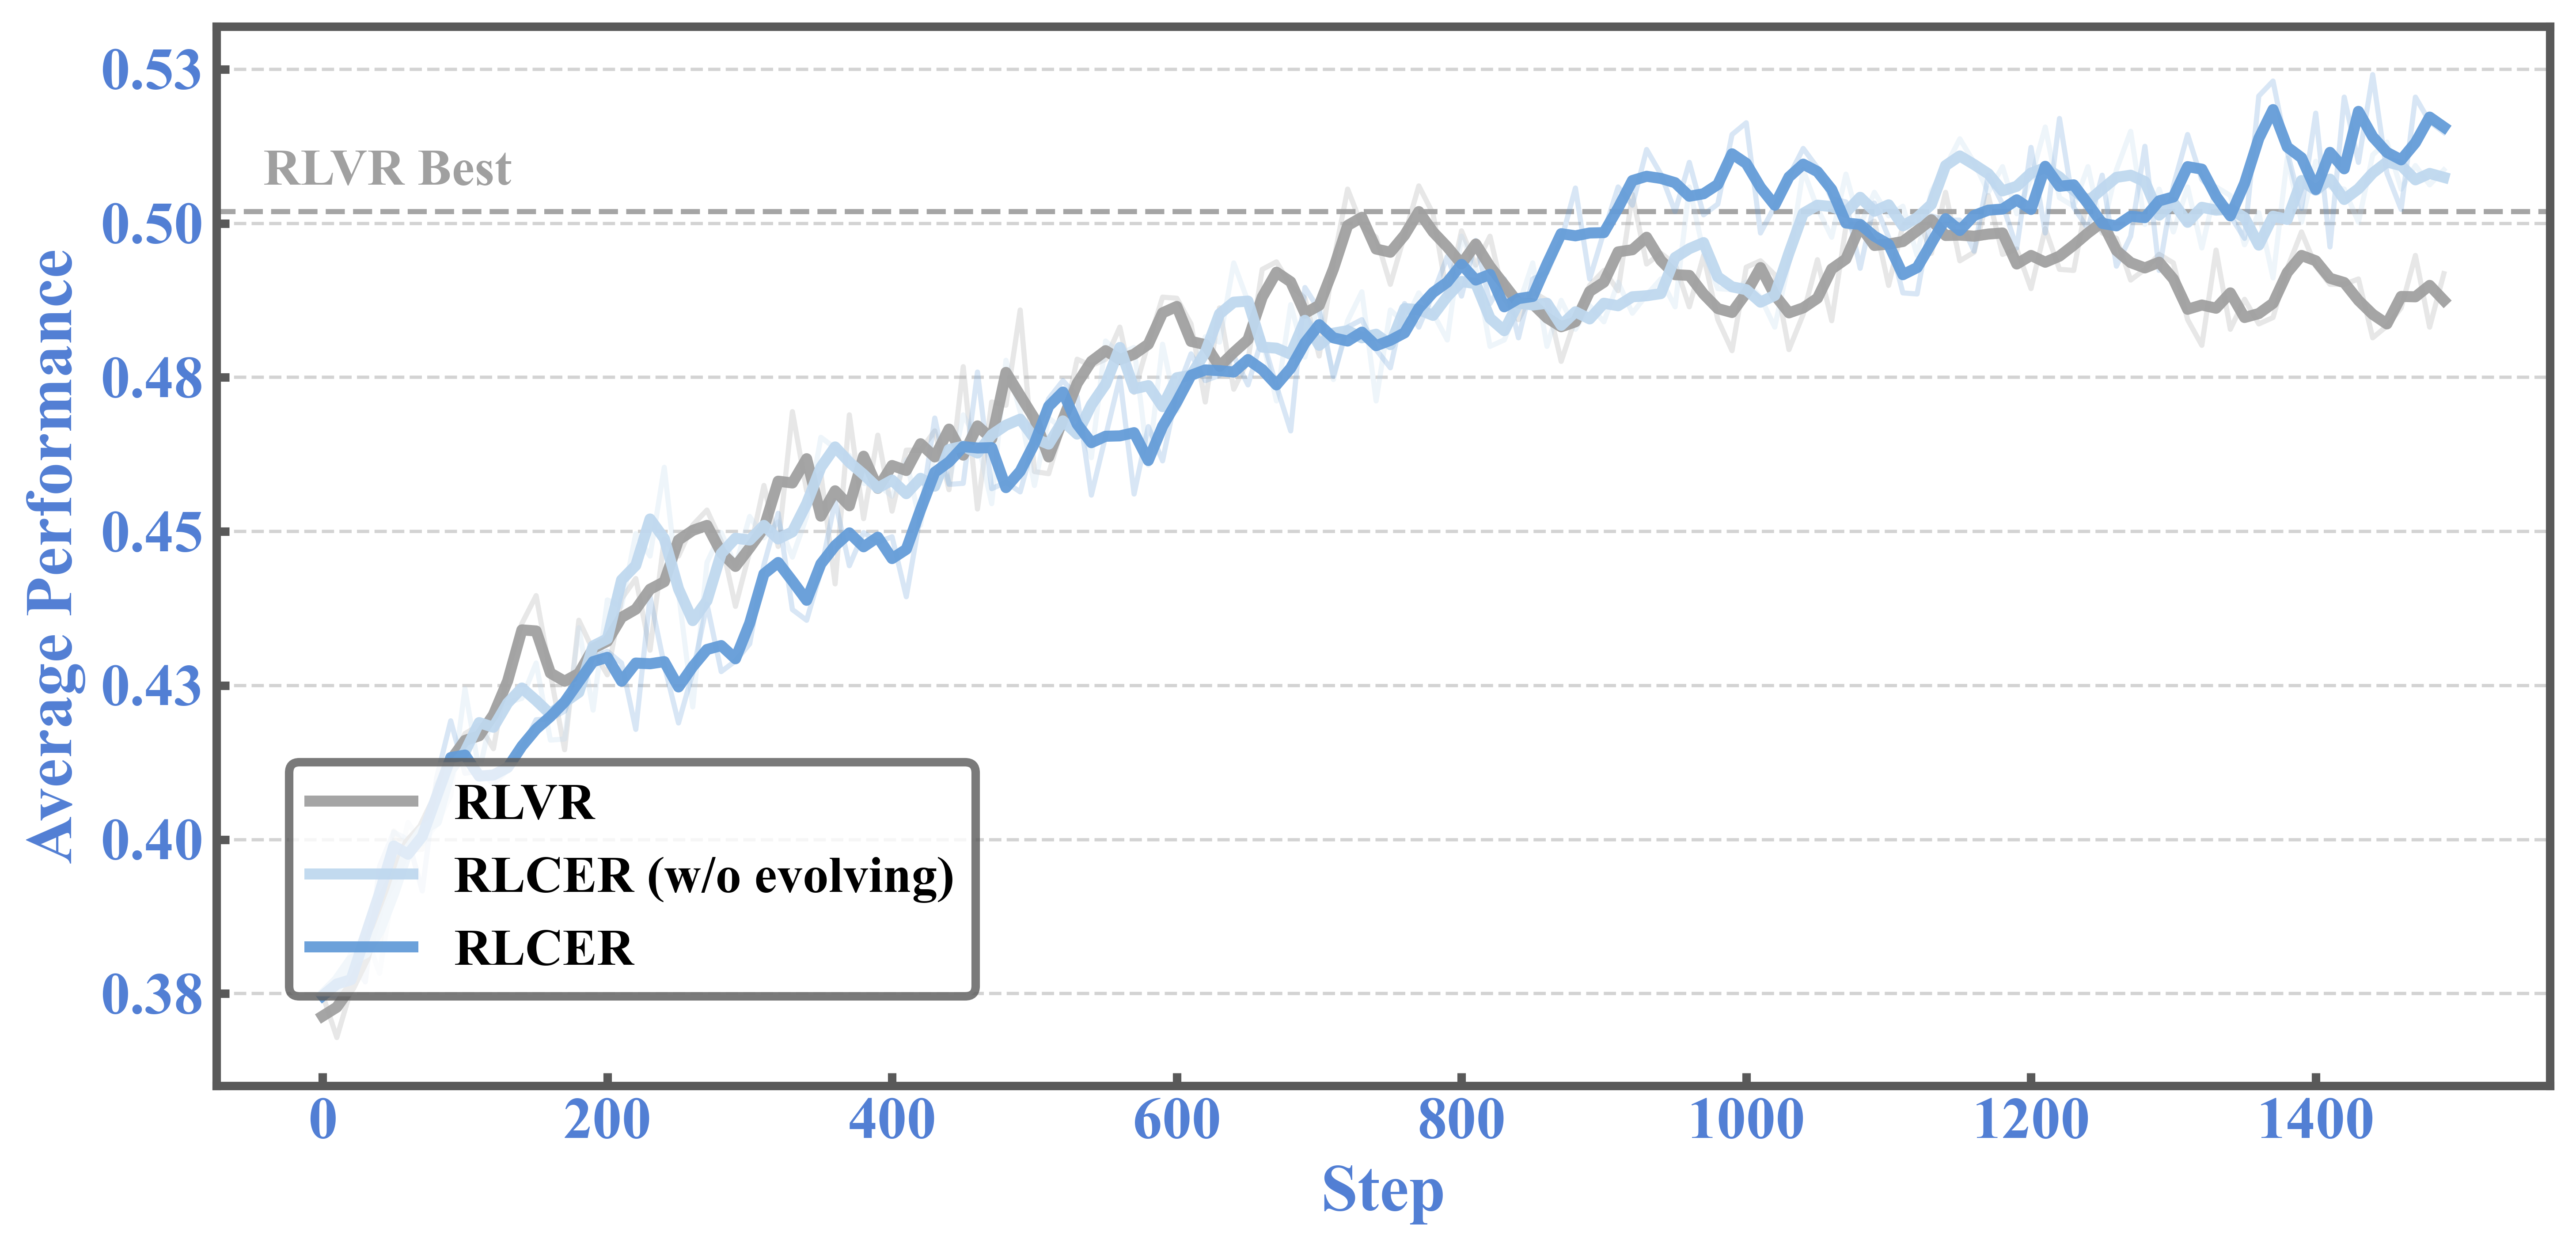
\includegraphics[width=\linewidth]{figures/exp/evolving_ablation/evolving_abl_perf.png}
        \vspace{-20pt}
        \caption{Average performance dynamics.}
        \label{fig:ablation-perf-dynamics}
    \end{subfigure}
    \begin{subfigure}[t]{0.382\columnwidth}
        \centering
        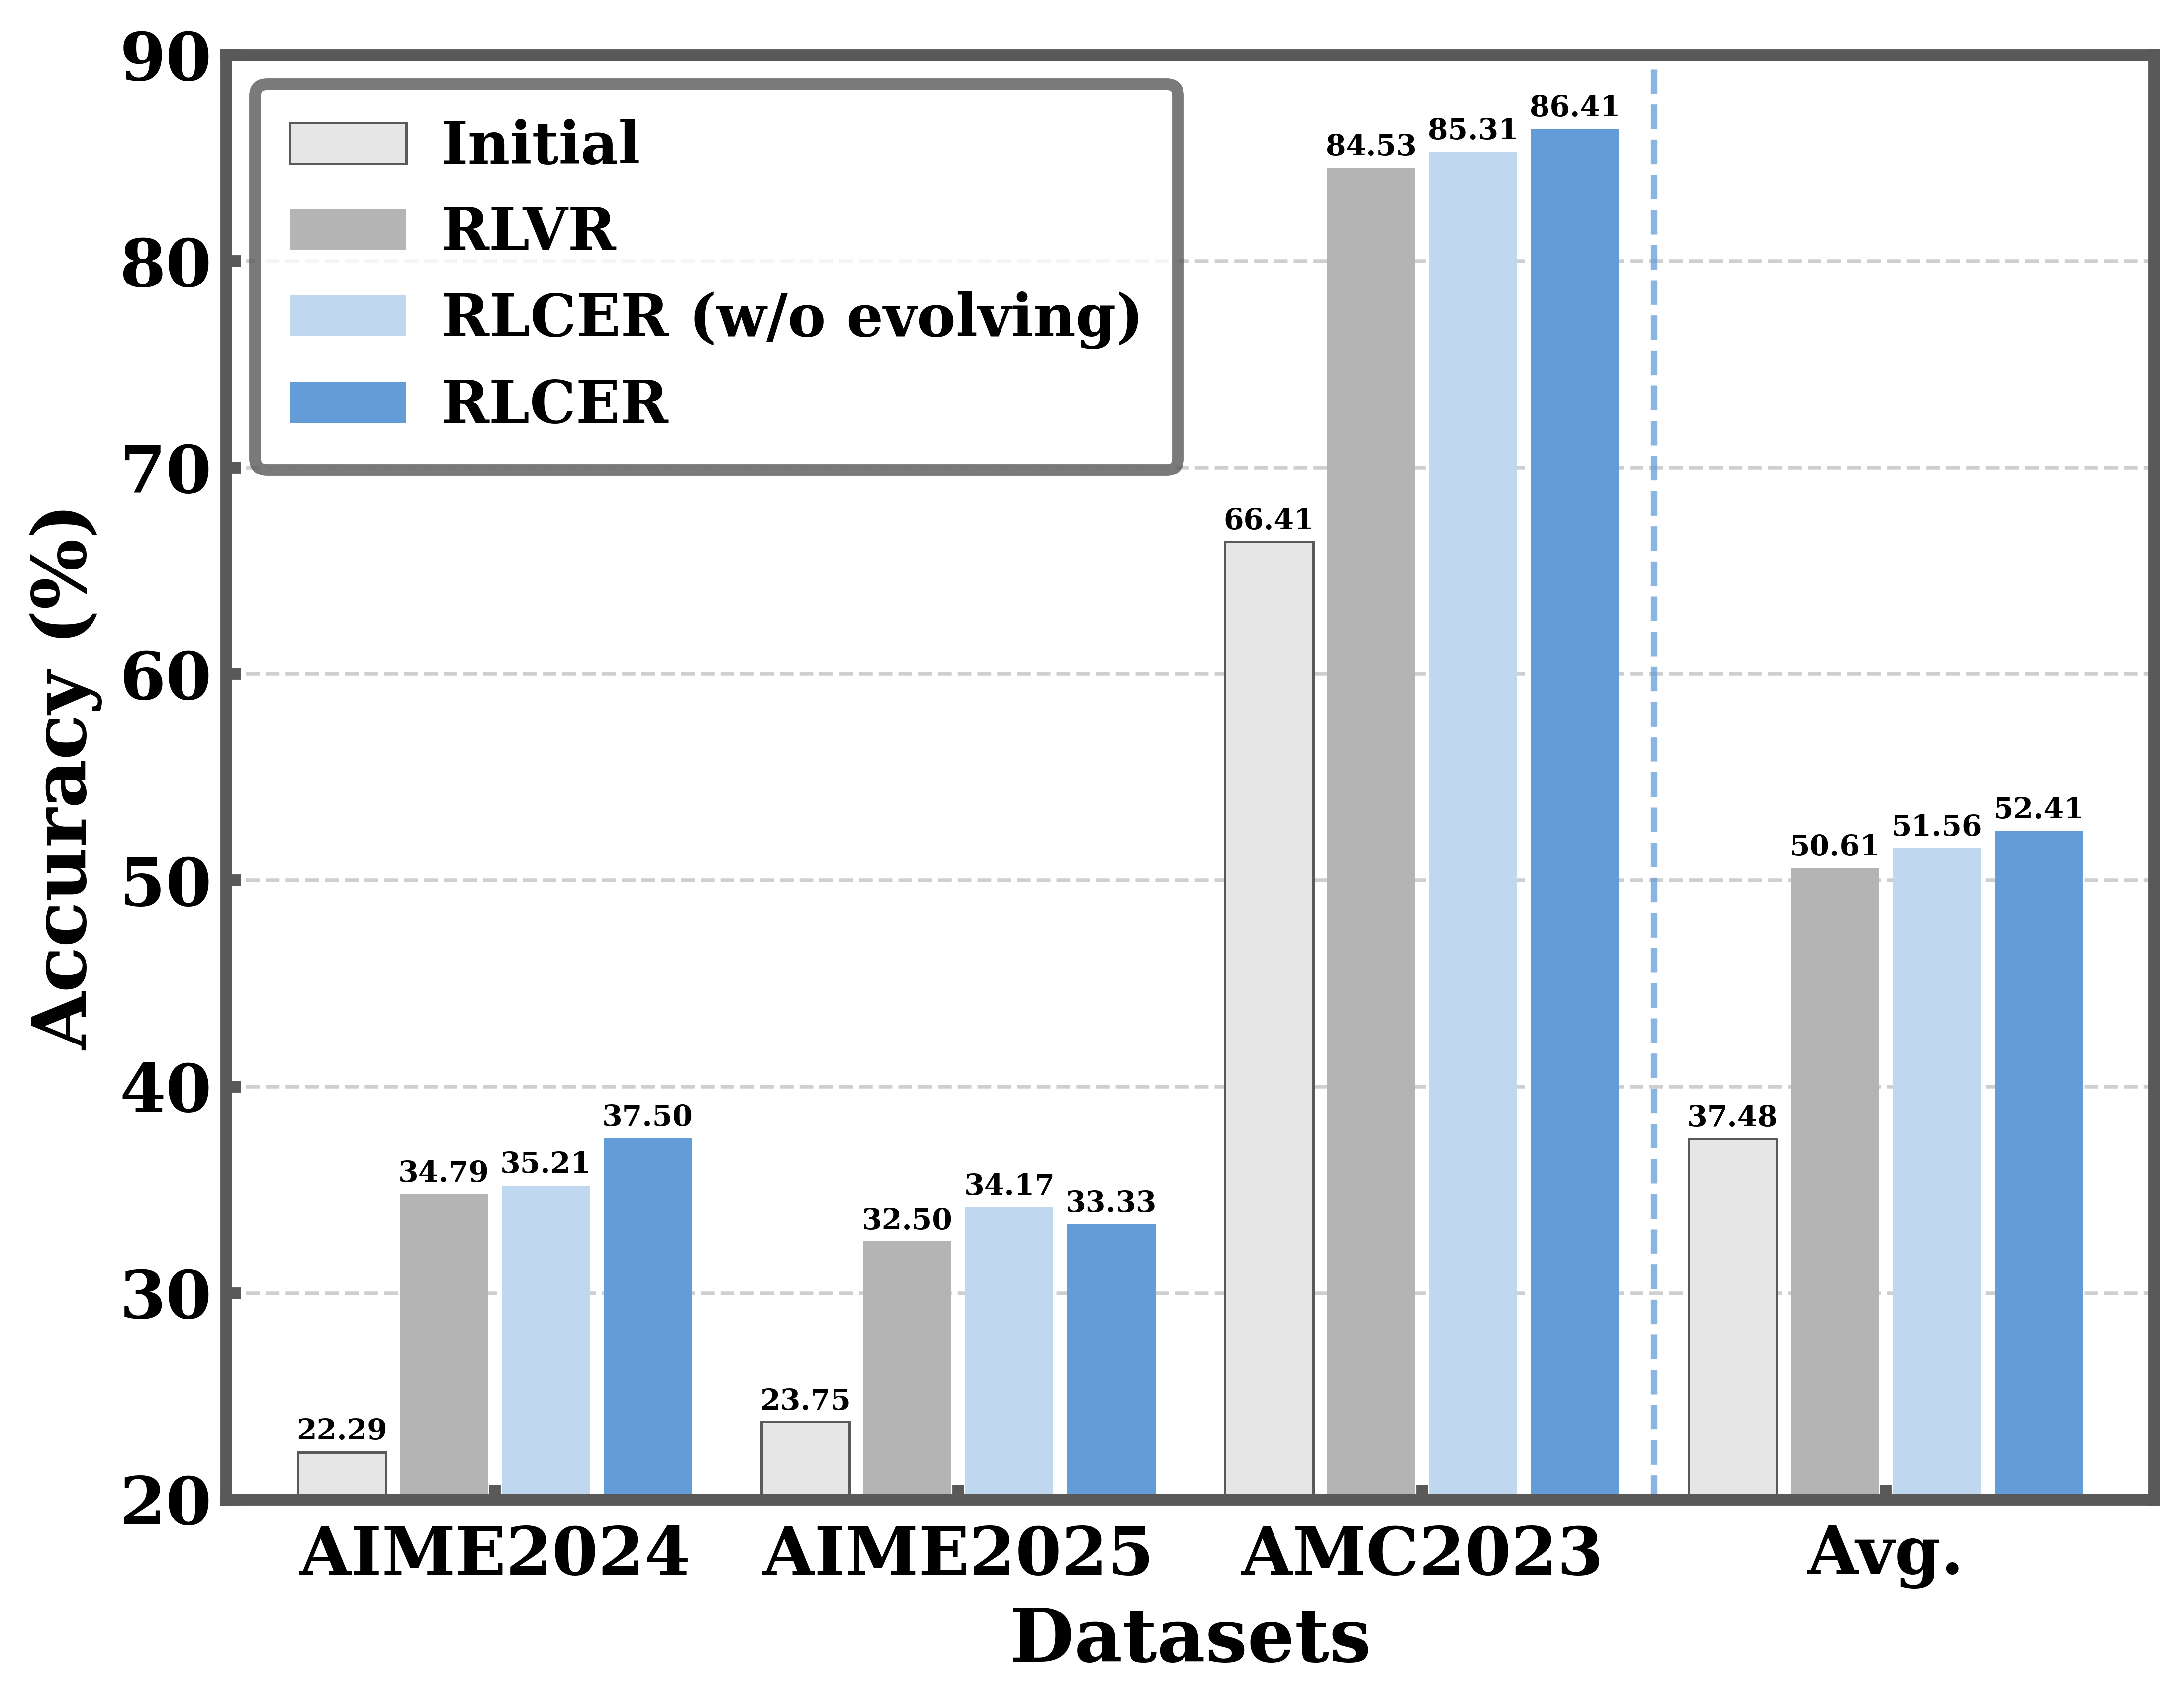
\includegraphics[width=\linewidth]{figures/exp/evolving_ablation/abl_perf.png} % ABLperf
        \vspace{-20pt}
        \caption{Performance comparison.}
        \label{fig:ablation-perf-final}
    \end{subfigure}
    \vspace{-8pt}
    \caption{Performance across three math datasets on the 7B model. Training with RLCER leads to a higher performance ceiling, and the self-evolving rubrics further enhance reasoning performance. }
    \label{fig:ablation-perf}
\end{figure}




\clearpage
\section{Introduction}


\begin{figure}[ht]
    \centering
    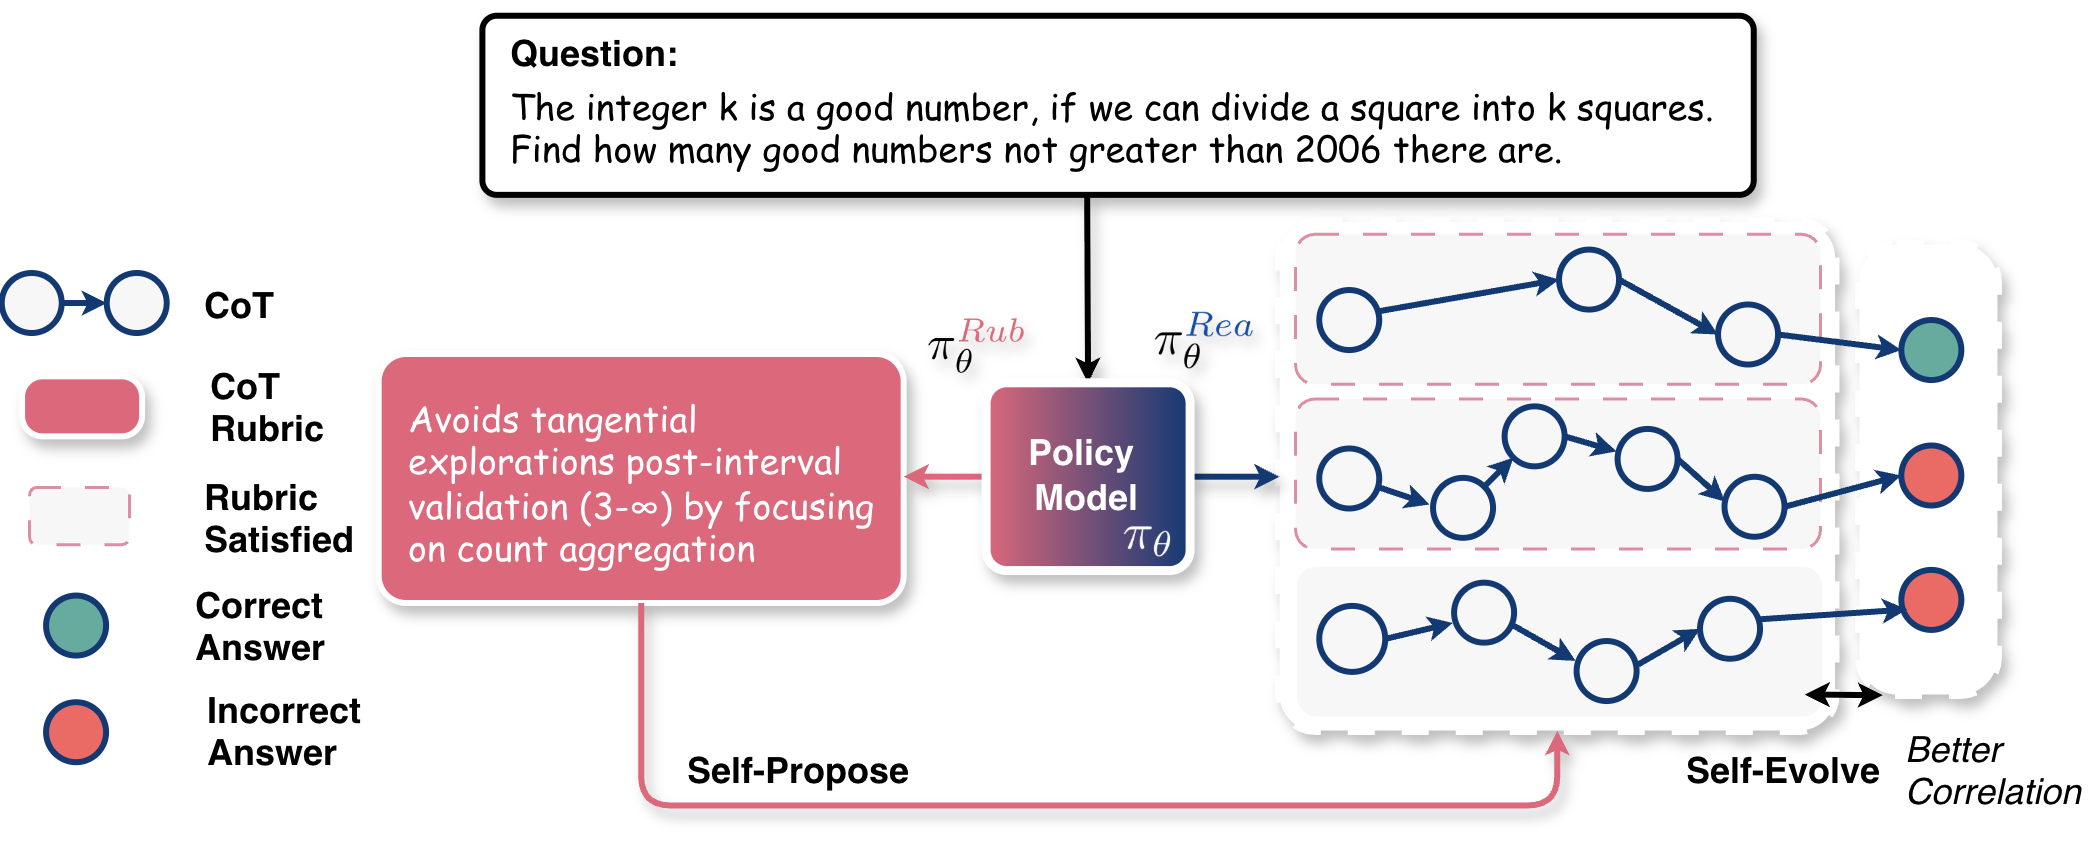
\includegraphics[width=0.9\columnwidth]{figures/framework/RLCER_teaser.png}
    \vspace{-8pt}
    \caption{Key idea of reinforcement learning with CoT supervision via self-evolving rubrics (RLCER). The policy model $\pi_\theta$ acts as both the reasoner and the rubrics generator, self-generating and self-evolving the rubrics for CoT supervision, where the evolving direction is shaped towards the correlation with the rubrics satisfaction and the final answer correctness.}
    \label{fig:teaser-figure}
    \vspace{-6pt}
\end{figure}


Chain-of-thought (CoT) \cite{CoT} reasoning is essential for large language models (LLMs) to solve complex tasks, where its quality strongly affects the final-answer correctness \cite{Demystifying-CoT, what-characterizes-cot, LCoT2Tree, ProcessBench}. 
However, CoT is rarely rewarded or optimized explicitly, even often regarded as a by-product of outcome-centric optimization objectives in large-scale reinforcement learning with verifiable rewards (RLVR) \cite{Deepseek-R1, O1, DeepSeekMath}.
This yields an underconstrained learning signal: for the same final answer, many distinct reasoning trajectories receive identical rewards, allowing optimization to drift toward shortcut or brittle strategies \cite{RuscaRL, zhang2025interplay}. Consequently, the model can converge to sub-optimal reasoning behaviors, limiting robustness and overall capability \cite{PRM8K}.

\revision{However, while important, directly rewarding or supervising CoTs remains challenging in practice, mainly for two reasons:}
(i) training additional reward models (RMs) for CoT supervision typically requires labor-intensive and fine-grained annotations \cite{PRM8K, PRIME}, 
and (ii) the policy’s CoT distribution shifts during training, yielding non-stationary and potentially biased supervision. 
\textit{\textbf{Can the policy model \concept{self-propose} rubrics as CoT supervision criteria and self-evolve them during training with no human annotations?}} 
If so, this could enable a new paradigm of self-improving reasoning, shifting RL from optimizing \concept{what LLMs answer} to autonomously improving \concept{how LLMs think}, potentially yielding \concept{``free-lunch''}  reasoning gains.

We find possibilities of achieving this from the recent advances in the research line of \concept{self-evolving training methods} \cite{self-evolving-survey, AlphaZero}, where a policy model $\pi_\theta$ can improve itself with little to no human intervention during training.
On the one hand, $\pi_\theta$ itself can self-generate training data, such as verifiable question-answer pairs for RL or high-quality CoT trajectories for cold-starting reasoning \cite{AbsoluteZero, SPICE, SSP, STaR}.
On the other hand, $\pi_\theta$ itself can self-assign reward signals by acting as a judge to evaluate its own solutions \cite{Self-Rewaring-Rubric, SRLM, SeRL, SPIN}.
A key idea shared by these methods is to let a single policy model $\pi_\theta$ play multiple roles under different prompts, serving not only as a reasoner that produces solutions but also as a data generator or a reward provider \cite{AbsoluteZero, SRLM}, with all roles optimized jointly (\eg via techniques such as multi-agent reinforcement learning \cite{AbsoluteZero}). 
Together, these capabilities make it plausible to self-propose supervision criteria (\eg rubrics) for assessing CoT quality and to self-evolve as training progresses.
However, how to adaptively propose and evolve such criteria in the self-evolving training paradigm remains largely underexplored.

To fill this gap, we propose \textbf{RLCER} (\textbf{R}einforcement \textbf{L}earning with \textbf{C}oT Supervision via Self-\textbf{E}volving \textbf{R}ubrics), empowering RLVR with self-proposed and self-evolving rubrics to supervise CoT reasoning.
The core idea is to let the policy model $\pi_\theta$ self-propose CoT supervision criteria as natural-language rubrics (\ie describing desirable reasoning properties like ``avoid tangential explorations'')
\cite{Rubrics-as-Rewards, Chasing-the-Tail}, rewarding CoTs by their rubric satisfaction, and simultaneously improving the model’s rubric-generation ability throughout training.
An overview of the key process is illustrated in Figure~\ref{fig:teaser-figure}.
Specifically, a single policy model $\pi_\theta$ is instantiated with different prompts to play two roles: a reasoner $\pi_{\theta}^{\text{\textcolor{reasoner}{$Rea$}}}$ that generates CoTs $\hat{\mathcal{C}}$ and final answers $\hat{\mathcal{A}}$, and a rubricator $\pi_{\theta}^{\text{\textcolor{rubricator}{$Rub$}}}$ that generates a set of candidate rubrics $\hat{\mathcal R} \triangleq \{\hat{\tau}_k\}_{k=1}^{K}$, where $K$ is the number of rubrics $\hat{\tau}_k$. 
The reasoner is rewarded by both the final answer correctness and the CoT quality, which is measured by satisfaction of all valid rubrics $\hat{\tau}^{valid}_k$. 
Here, we deem a rubric $\hat{\tau}_k$ valid if its satisfaction indicator $\mathbf v_k$ is strongly correlated with final-answer correctness $\mathbf z$ across multiple sampled rollouts for the same question $\mathcal Q$ (\ie $\mathtt{corr}(\mathbf v_k,\mathbf z)>\alpha$), since a high correlation means that satisfying the rubric aligns with producing correct answers. 
Additionally, we encourage the rubricator to self-evolve its rubric generation capability by rewarding the fraction of valid rubrics among its proposals
 (\ie $\frac{|\{\hat{\tau}^{valid}_k\}|}{K}$). 

Generally, RLCER enables RLVR to move beyond outcome-centric optimization by rewarding CoTs with supervision criteria that are self-proposed and self-evolved, without any human annotation.
We further conduct comprehensive experiments to examine the effectiveness of the proposed RLCER. 
First, we conduct a primary study showcasing that self-proposed rubrics can be reliable and learnable even when training is driven solely by rubric-based rewards, without any outcome reward (\cf Section \ref{sec:rubrics-reliability}). 
Based on this insight, RLCER generally outperforms the naive RLVR (\cf Section \ref{sec:main-performance}). 
Additionally, introducing self-evolving training for the rubricator further improves the reasoning performance (\cf Section \ref{sec:rubrics-self-evolving}).
Moreover, the generated rubrics can even serve as in-prompt hints to enhance reasoning at inference time (\cf Section \ref{sec:rubrics-as-hint}).
Overall, our results suggest a new paradigm in which models autonomously generate CoT supervision criteria to strengthen RL training, pointing toward more self-improving and self-evolving reasoning systems. 

\section{Related Works}
\subsection{LLM Reasoning with RL}
Reinforcement learning has become an essential technique for incentivizing chain-of-thought (CoT) reasoning in LLMs \cite{RL4LRM, Survey-LLMs}.
A milestone paradigm is reinforcement learning with verifiable rewards (RLVR) \cite{DeepSeekMath, O1, Deepseek-R1}, where LLMs are trained on verifiable tasks such as math problems \cite{AIME}, puzzle solving \cite{ARC-AGI-2}, and code execution \cite{LiveCodeBench}, by rewarding final-answer correctness using task-specific verifiers.
Since such tasks are intrinsically difficult to reward-hack, RLVR tends to encourage LLMs to produce longer CoTs before answering, thereby improving reasoning performance \cite{Deepseek-R1, O1}.
However, despite its effectiveness in incentivizing reasoning, most RLVR training remains outcome-centric and provides no direct supervision over the CoT itself, lacking guidance on how the model should reason.
While several efforts have tried to mitigate this by assigning process rewards using additional reward models (RM) \cite{PRM8K}, training such RMs requires labor-intensive training data collection \cite{PRM8K, PRIME, ProcessBench}, and a static RM often fails to keep pace with the evolving CoT distribution during training \cite{Deepseek-R1}.
Therefore, such challenges hinder the combination of RLVR training with CoT supervision criteria for rewarding in practice.

\subsection{Self-Evolving in LLMs}
A critical step toward general artificial intelligence lies in the ability to self-evolve with little or no human intervention \cite{self-evolving-survey}. 
Recent work has made progress via self-training and self-play, where a single policy model $\pi_\theta$ can self-generate training data \cite{AbsoluteZero, SSP, SPICE}, or self-provide reward signals during learning \cite{SPIN, SeRL, SRLM}. 
The self-evolving capabilities can further be strengthened with techniques such as multi-role reinforcement learning, where a single policy model $\pi_\theta$ is prompted to play different roles (\eg reasoner, data generator, or reward provider) and trained with role-specific rewards \cite{AbsoluteZero, SPICE, Alignmen-Waltz}.
Therefore, these advances in such self-evolving methods suggest the possibilities of self-proposing criteria for CoT supervision, while this direction remains largely under-explored.

\subsection{Reinforcement Learning with Rubrics}
Recently, reinforcement learning with rubrics has emerged as a promising way to provide fine-grained and interpretable reward signals \cite{Rubicon, Rubrics-as-Rewards, HealthBench, Chasing-the-Tail}.
Here, rubrics are structured, checkable evaluation criteria (\ie explicit requirements for assessing outputs) \cite{Rubrics-as-Rewards} that decompose high-level objectives into multi-facet supervision signals \cite{DR-Tulu}, enabling RL to extend towards non-verifiable and open-ended domains \cite{RuscaRL, Rubrics-as-Rewards}.
However, existing work largely applies rubrics to score response quality, leaving their effectiveness for CoT supervision underexplored.
Moreover, most approaches rely on predefined or static rubrics, which may become mismatched as model behaviors evolve during training \cite{DR-Tulu}.
To address these gaps, we introduce a framework that self-proposes rubrics as CoT supervision criteria and continually evolves them throughout training, integrating rubric-based RL for CoT supervision with self-evolving training.


\section{Preliminaries}
In this section, we briefly review the necessary background that forms the foundation of our work, including incentivizing LLM reasoning with RL in Section \ref{sec:pre-training} and multi-role RL under a single policy in Section \ref{sec:pre-masrl}. 

    \subsection{Incentivizing LLM Reasoning with RL} \label{sec:pre-training}
In this work, we focus on incentivizing LLMs to reason with RL, where the policy model is optimized by rewarding the high-quality rollouts.

\textbf{Rollout.}
Given a question $\mathcal{Q}$, the policy model $\pi_{\theta}$ attempts to solve it by generating a response that contains a CoT $\hat{\mathcal{C}}$ followed by an answer $\hat{\mathcal{A}}$, which can be formulated as:
\begin{equation}
\hat{\mathcal{C}}, \hat{\mathcal{A}} \sim \pi_{\theta}(\cdot \mid\mathcal{Q}).
\end{equation}
\textbf{Rewarding.}
After rollouts generation, rewards are assigned based on response quality, which can depend on: (i) the CoT $\hat{\mathcal{C}}$ and (ii) the answer $\hat{\mathcal{A}}$.
In the widely adopted RLVR paradigm, rewards typically depend solely on the correctness of the predicted answer $\hat{\mathcal{A}}$:
\begin{equation}\label{eq:outcome_reward}
r = \psi( \mathbb{I}(\mathcal{A},\hat{\mathcal{A}})),
\end{equation}
where $\mathbb{I}(\cdot,\cdot)$ is an answer correctness indication function which returns $1$ if two answers $\mathcal{A}$ and $\hat{\mathcal{A}}$ are equivalent and $0$ otherwise, and a reward assignment function $\psi$ maps this correctness signal $\mathbb{I}(\mathcal{A},\hat{\mathcal{A}})$ to a binary reward $r$.
Through such RLVR training, the policy model $\pi_\theta$ gradually learns to answer questions, which is often associated with producing longer CoTs \cite{Deepseek-R1}.
% thereby achieving higher answer accuracy.
However, under the RLVR paradigm, the CoT $\hat{\mathcal{C}}$ itself is rarely rewarded directly due to practical implementation challenges \cite{Deepseek-R1}, while the lack of such supervision may induce sub-optimal reasoning strategies \cite{PRM8K}.

\subsection{Multi-Role RL Under a Single Policy Model} \label{sec:pre-masrl}
Recently, studies have shown that a single policy model $\pi_\theta$ can effectively learn multiple roles by assigning role-specific rewards \cite{AbsoluteZero, SPIRAL}:
\begin{equation}\label{eq:reward-role}
r^{\text{role}_i} \rightarrow \pi^{\text{role}_i}_\theta,
\end{equation}
where $r^{\text{role}_i}$ denotes the reward assigned to $\text{role}_i$, and $\pi^{\text{role}_i}_\theta$ represents the same underlying policy model $\pi_\theta$ instantiated under the prompt $\mathcal{P}^{\text{role}_i}$ corresponding to that role.

A typical application under this framework is to let the model simultaneously act as a reasoner and a data generator, achieving RL training starting from no human-labeled data \cite{AbsoluteZero, AlphaZero, SSP}. 
More broadly, this multi-role, single-policy setup provides a natural substrate for self-evolving training: different roles instantiated from the same model can compete \cite{AbsoluteZero, SPICE} or collaborate \cite{Alignmen-Waltz, SPIRAL}, continuously improving the learning signals and behaviors \cite{MAS-Survey}.
Building on this view, we investigate whether the same policy can simultaneously serve as a reasoner and a CoT rubrics generator (\ie rubricator). 
With role-specific rewards, the rubricator is encouraged to produce useful CoT supervision criteria, which in turn enables the self-evolution of CoT rewarding. 
In this case, the reasoner and rubricator collaborate together for better reasoning.



\section{Methodology}

In this section, we introduce \textbf{RLCER} (\textbf{R}einforcement \textbf{L}earning with \textbf{C}oT Supervision via Self-\textbf{E}volving \textbf{R}ubrics) for bootstrapping chain-of-thought reasoning. 
In the remainder of this section, we first briefly introduce the key idea of RLCER in Section \ref{sec:key-idea} to facilitate a high-level understanding. 
Then, we discuss the multiple roles under the same policy model in Section \ref{sec:roles}. 
After that, we discuss how to incentivize reasoning with self-proposed and rubrics in Section \ref{sec:reasoner_reward}. 
We then discuss how to self-evolve such rubrics in Section \ref{sec:reward_rubricator}.
Finally, we present how to optimize the policy $\pi_\theta$ under the two roles based on role-specific rewards in Section \ref{sec:policy-optimization}.

\subsection{Key Idea} \label{sec:key-idea}
\begin{wrapfigure}{r}{0.48\textwidth}
    \centering
    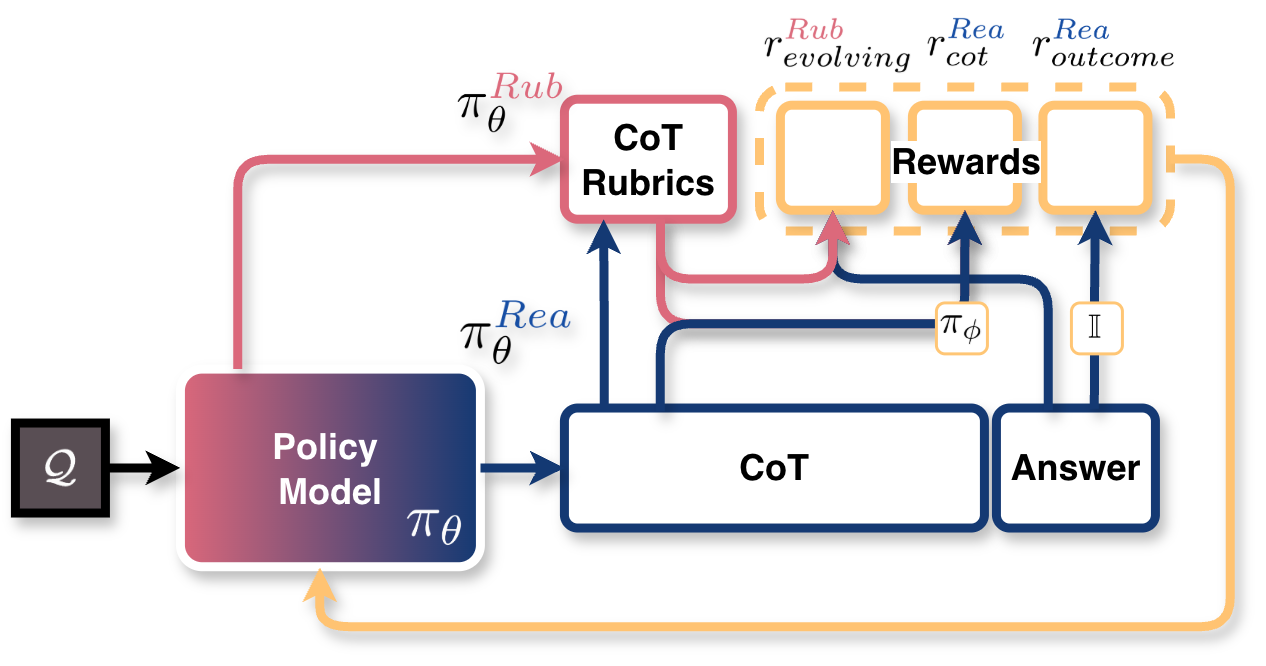
\includegraphics[width=\linewidth]{figures/framework/RLCER_key_idea.png}
    \vspace{-14pt}
    \caption{The RLCER loop. Format reward is ignored for brevity. One single policy model self-proposes rubrics for rewarding CoTs, and self-evolves the rubrics via rewarding generation capabilities.}
    \vspace{-8pt}
    \label{fig:key-idea}
\end{wrapfigure}

The key idea of RLCER is to go beyond rewarding what LLMs answer (\ie final-answer correctness) to explicitly and autonomously reward how LLMs think (\ie CoT quality) using self-proposed, self-evolving rubrics. The rubrics are evolved by tracking how well their satisfaction correlates with the final answer correctness.

To achieve this goal, we introduce two key roles in the multi-role RL framework for optimization: the reasoner $\pi_{\theta}^{\text{\textcolor{reasoner}{$Rea$}}}$ for answering the question and the rubricator $\pi_{\theta}^{\text{\textcolor{rubricator}{$Rub$}}}$ for generating rubrics supervising CoTs.
Here, the reasoner $\pi_{\theta}^{\text{\textcolor{reasoner}{$Rea$}}}(\cdot)=\pi_{\theta}(\cdot\mid\mathcal{P}^{\text{\textcolor{reasoner}{$Rea$}}})$ and the rubricator $\pi_{\theta}^{\text{\textcolor{rubricator}{$Rub$}}}(\cdot)=\pi_{\theta}(\cdot\mid\mathcal{P}^{\text{\textcolor{rubricator}{$Rub$}}})$ share the same policy parameter $\theta$, while their roles are distinguished by different prompts $\mathcal{P}^{\text{\textcolor{reasoner}{$Rea$}}}$ and $\mathcal{P}^{\text{\textcolor{rubricator}{$Rub$}}}$ respectively. 
The prompts can be found in Appendix \ref{apdx:prompts}. 
Additionally, a verifier $\pi_\phi$ is used for judging the satisfaction of rubrics, which is another fine-tuned and frozen model parameterized by $\phi$. 

As shown in Figure \ref{fig:key-idea}, we explicitly refine how the reasoner $\pi_{\theta}^{\text{\textcolor{reasoner}{$Rea$}}}$ thinks, by rewarding the CoT quality beyond the answer correctness, with the CoT quality evaluated by the verifier $\pi_\phi$ based on rubrics generated by the rubricator. 
We further enable rubric generation to self-evolve for more autonomous and effective CoT supervision by rewarding the quality of generated rubrics, guided by the correlation between rubric satisfaction degree and answer correctness.
We jointly optimize the policy model $\pi_\theta$ under two roles by assigning different rewards for each role. 
After computing role-specific rewards, we optimize the shared policy model $\pi_\theta$ for both roles, with advantages computed separately for each role \cite{SPICE}.


\subsection{Two Roles in One Policy: Reasoner and Rubricator} \label{sec:roles}
In this section, we take a closer look at the different roles of the reasoner $\pi_{\theta}^{\text{\textcolor{reasoner}{$Rea$}}}$ and the rubricator $\pi_{\theta}^{\text{\textcolor{rubricator}{$Rub$}}}$, within the RLCER framework.

\textbf{Reasoner} $\pi_{\theta}^{\text{\textcolor{reasoner}{$Rea$}}}$. 
The reasoner answers the question by generating a CoT $\hat{\mathcal C}$ and a final answer $\hat{\mathcal A}$.
Given the question $\mathcal Q$, the rollout sampling process of the reasoner can be formulated as:
\begin{equation}
\hat{\mathcal C}, \hat{\mathcal A} \sim 
\pi_{\theta}^{\text{\textcolor{reasoner}{$Rea$}}}\!\big(\cdot \mid \mathcal Q\big),
\end{equation}
where $\hat{\mathcal C}$ denotes the CoT process, and $\hat{\mathcal A}$ denotes the predicted final answer.

\textbf{Rubricator} $\pi_{\theta}^{\text{\textcolor{rubricator}{$Rub$}}}$.
The rubricator generates a set of $K$ rubrics for evaluating the CoT qualities based on the question $\mathcal Q$ and one CoT $\hat{\mathcal C}$. 
Given the question $\mathcal Q$ and a generated CoT $\hat{\mathcal C}$, the rollout sampling process of the rubricator can be formulated as:
\begin{equation}
\hat{\mathcal R} \sim 
\pi_{\theta}^{\text{\textcolor{rubricator}{$Rub$}}}
\big(\cdot \mid \mathcal Q, \hat{\mathcal C}\big),
\qquad
\hat{\mathcal R} \triangleq \{\hat{\tau}_k\}_{k=1}^{K},
\ \hat{\tau}_k \triangleq (\hat c_k,\hat s_k).
\end{equation}
The generated textual output $\hat{\mathcal R}$ contains $K$ specific rubrics, each denoted as $\hat{\tau}_k$. Here, $\hat c_k$ is the textual criterion (\eg ``avoids tangential explorations post-interval validation (3-$\infty$) by focusing on count aggregation'') of rubric $\hat{\tau}_k$ and $\hat s_k \in \mathbb{R}$ is the score of rubric $\hat{\tau}_k$ reflecting its importance, which can be both positive or negative. 
The rubrics generated under the rubricator role will then be used for judging the CoT quality through an external verifier $\pi_\phi$.

\subsection{Rewarding How to Think via Self-Proposed Rubrics} \label{sec:reasoner_reward}
In this section, we discuss how to autonomously reward how LLMs think via self-proposed rubrics. 

\textbf{Rewarding CoT with self-proposed rubrics.} Specifically, we reward a CoT based on how well it satisfies the valid rubrics proposed by the rubricator $\pi_{\theta}^{\text{\textcolor{rubricator}{$Rub$}}}$.
The CoT reward is computed by aggregating the scores of the satisfied rubrics:
\begin{equation}
    r_{cot}^{\text{\textcolor{reasoner}{$Rea$}}}=\texttt{norm}\left(\sum_{\hat{\tau}_{k} \in \hat{\mathcal{R}}_{valid}}\pi_\phi \left(\hat c_k, \hat{\mathcal{C}}\right)\cdot\hat s_k\right),
\end{equation}

where $\hat{\mathcal{R}}_{valid}$ denotes the set of valid rubrics from the rubricator, $\pi_\phi(\hat c_k, \hat{\mathcal{C}})\in\{0,1\}$ is a binary value produced by the verifier $\pi_\phi$ indicating whether the CoT $\hat{\mathcal{C}}$ satisfies rubric $\hat c_k$, and $\texttt{norm}(\cdot)$ is a normalization function that maps the aggregated score to the interval $[0,1]$. The function $\texttt{norm}(\cdot)$ conducts the min–max normalization as $\texttt{norm}(x) = (x-\text{MinValue}) / (\text{MaxValue}-\text{MinValue})$, where MinValue and MaxValue denote the minimum and maximum aggregated rubric scores attainable under the valid rubrics $\hat{\mathcal{R}}_{valid}$, respectively.

\textbf{Valid rubrics}. Here, a rubric $\hat{\tau}_k$ is considered valid if it is informative as a rewarding criterion: 
(i) its satisfaction indicator $\mathbf v_k$ is positively correlated with final-answer correctness $\mathbf z$
across $N$ sampled rollouts of the same question $\mathcal Q$ (\ie $\mathtt{corr}(\mathbf v_k,\mathbf z)>\alpha$),
and (ii) it is discriminative across different CoTs and would not yield consistent satisfaction (\ie $\mathtt{std}(\mathbf v_k)>0$). 
We define $\mathbf v_k$ and $\mathbf z$ over these $N$ rollouts as:
\begin{equation}
\begin{aligned}
\mathbf v_k &\triangleq \Big[\pi_\phi(\hat c_k,\hat{\mathcal C}_0),\ldots,\pi_\phi(\hat c_k,\hat{\mathcal C}_N)\Big],\\
\mathbf z   &\triangleq \Big[\mathbb{I}(\mathcal A,\hat{\mathcal A}_0),\ldots,\mathbb{I}(\mathcal A,\hat{\mathcal A}_N)\Big].
\end{aligned}
\end{equation}

The intuition is that higher correlation implies that satisfying the rubric is consistently associated with correct final answers and can produce informative rewarding signals. Here $\alpha$ is set as 0.2 by default in our paper. 

\textbf{Outcome reward.} The CoT reward $r_{cot}^{\text{\textcolor{reasoner}{$Rea$}}}$ can be used as an auxiliary reward alongside the outcome reward $r^{\text{\textcolor{reasoner}{$Rea$}}}_{outcome}$, which is calculated as follows:
\begin{equation}\label{eq:outcome_reward}
r^{\text{\textcolor{reasoner}{$Rea$}}}_{outcome} =  
\begin{cases}
  1, & \texttt{is\_equiv}(\mathcal{A},\hat{\mathcal{A}})\\
  -1, & \text{Otherwise.}
\end{cases}
\end{equation}

Following DAPO \cite{DAPO}, we assign a binary outcome reward based on final answer correctness: $r^{\text{\textcolor{reasoner}{$Rea$}}}_{outcome}$=1 if the predicted answer $\hat{\mathcal{A}}$ is equivalent to the ground truth answer $\mathcal{A}$, and $r^{\text{\textcolor{reasoner}{$Rea$}}}_{outcome}$=-1 otherwise. 

\textbf{Total reward for reasoner.} Finally, the overall reward for the reasoner is the combination of the outcome reward and the CoT reward:

\begin{equation}
r^{\text{\textcolor{reasoner}{$Rea$}}} = 
    r^{\text{\textcolor{reasoner}{$Rea$}}}_{outcome} + r_{cot}^{\text{\textcolor{reasoner}{$Rea$}}}.
\end{equation}

Such a reward enables autonomously optimizing what LLMs answer and how LLMs think simultaneously. 

\subsection{Rubrics Self-Evolving for Better Supervision} \label{sec:reward_rubricator}
While the two-role design enables a single policy model to self-propose rubrics for CoT supervision, we argue that such rubrics may get saturated: once consistently satisfied by all rollouts, they lose discriminative power over CoT quality and no longer provide reward signals, as shown in Section \ref{sec:reasoner_reward}. 
Therefore, we further propose to self-evolve the rubric generation capability, so as to progressively produce more informative and challenging rubrics that mitigate saturation.

\textbf{Self-evolving with validity reward.} To achieve rubricator self-evolving, we reward the fraction of the number of valid rubrics among all generated rubrics as follows: 
\begin{equation}
r_{evolving}^{\text{\textcolor{rubricator}{$Rub$}}}=\frac{K_{\text{valid}}}{K},
\end{equation}

% \clearpage
where $K$ and $K_{\text{valid}} \triangleq |\{\hat{\tau}^{valid}_k\}|$ are the numbers of all generated rubrics and valid rubrics, respectively. 
Such rewards encourage the rubricator to generate more informative rubrics that are positively correlated with answer correctness (\ie $\mathtt{corr}(\mathbf v_k,\mathbf z)>\alpha$) and discriminative (\ie $\mathtt{std}(\mathbf v_k) > 0$), thereby preventing rubric saturation. 
This reward provides a simple way for evolving the quality of generated rubrics, by connecting the satisfaction of the rubrics with the final answer correctness.

\textbf{Format reward.} Additionally, to ensure the proposed rubrics can be stably parsed, we reward the rubricator with a format reward, rewarding the correct format as follows:

\begin{equation}
    r_{format}^{\text{\textcolor{rubricator}{$Rub$}}}=\begin{cases}
  1, & \text{The format is correct.}\\
  0, & \text{Otherwise.}
\end{cases}
\end{equation}

\textbf{Total reward for rubricator.} Finally, the total reward for the rubricator is calculated as the combination of the quality reward and the format reward:

\begin{equation}
   r^{\text{\textcolor{rubricator}{$Rub$}}} =  r_{evolving}^{\text{\textcolor{rubricator}{$Rub$}}} + r_{format}^{\text{\textcolor{rubricator}{$Rub$}}}.
\end{equation}

Such a reward design encourages the rubricator to continuously refine its proposed rubrics, consistently providing informative rewarding signals for CoT supervision.  

\begin{figure*}[t]
    \captionsetup{justification=raggedright,singlelinecheck=false}
    \centering
    \scalebox{1}[1]{%
        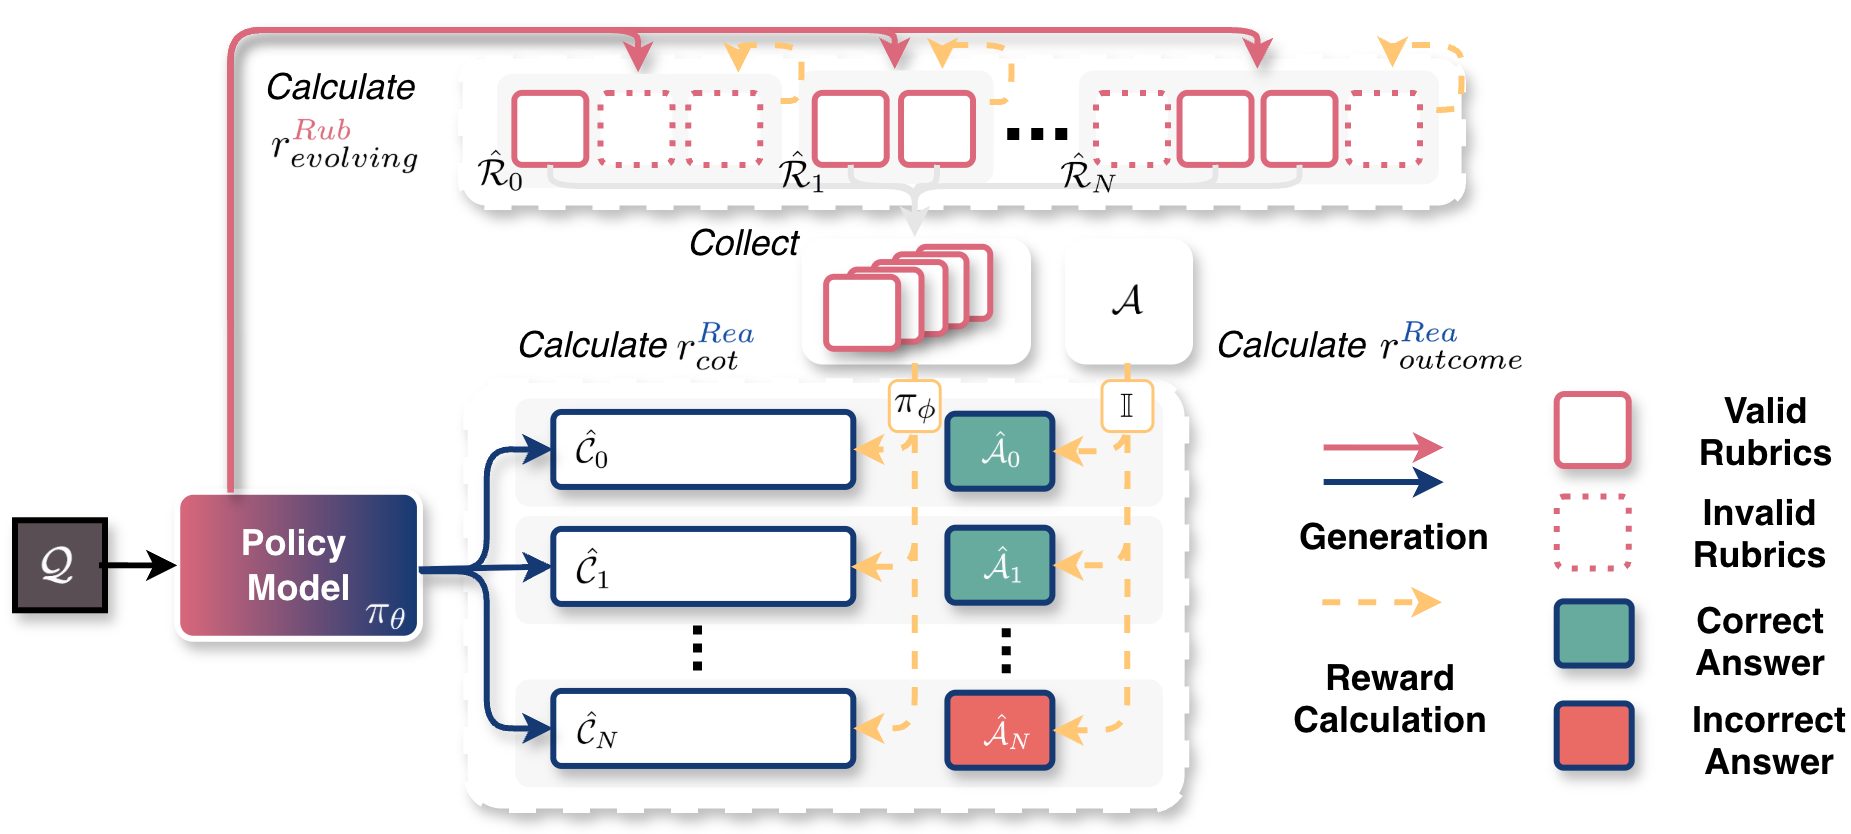
\includegraphics[width=0.88\textwidth]{figures/framework/RLCER_main_figure.png}%
    }
    \vspace{-6pt}
    \caption{Illustration of the reward calculation process in RLCER. For question $\mathcal{Q}$, the reasoner generates $N$ responses each with CoT $\hat{\mathcal{C}}_k$ and the final answer $\hat{\mathcal{A}}_k$. 
    After that, the rubricator generates $K_{n}$ specific rubrics (\ie $\hat{\mathcal R}_n \triangleq \{\hat{\tau}_k\}_{k=1}^{K_n}$). 
    The outcome reward is applied first by matching the generated answer $\hat{\mathcal{A}}_k$ with the ground-truth answer $\mathcal{A}$.
    All the valid rubrics (\ie $\mathtt{corr}(\mathbf v_k,\mathbf z)>\alpha$ and $\mathtt{std}(\mathbf v_k)>0$) are collected for rewarding CoTs. 
    And the fraction of valid rubrics for the $k$-th rubricator generation (\ie $\frac{|\{\hat{\tau}^{valid}_{n,k}\}|}{K_n}$) is used for rewarding the rubricator to self-evolve. 
    }
    \label{fig:main-figure}
    % \vspace{-6pt}
\end{figure*}


\subsection{Two-Role Optimization under a Single Policy} \label{sec:policy-optimization}

After computing the rewards for the reasoner and the rubricator, we jointly optimize the shared policy model $\pi_\theta$ under both roles in an end-to-end manner. Specifically, we compute role-specific advantages $\hat{A}^{\text{\textcolor{reasoner}{$Rea$}}}_t$ and $\hat{A}^{\text{\textcolor{rubricator}{$Rub$}}}_t$  from their respective rewards $r^{\text{\textcolor{reasoner}{$Rea$}}}$ and $r^{\text{\textcolor{rubricator}{$Rub$}}}$, and use them to update the policy via a standard policy-gradient objective. Gradients from both roles are aggregated to update the same set of parameters $\theta$, allowing the model to learn from role-specific feedback while maintaining a unified policy. The overall optimization procedure is illustrated in Algorithm~\ref{def:aglo}.

% \clearpage
With role-specific advantages $\hat{A}^{\text{\textcolor{reasoner}{$Rea$}}}_t$ and $\hat{A}^{\text{\textcolor{rubricator}{$Rub$}}}_t$, the optimization objective can be formulated as follows: 
\begin{equation}
\begin{aligned}
\mathcal{J}(\theta)
&= \ 
\mathbb{E}_{(\mathcal{Q}, \mathcal{A}) \sim \mathcal{D}^{\text{\textcolor{reasoner}{$Rea$}}},
\ \boldsymbol{o} \sim \pi^{\text{\textcolor{reasoner}{$Rea$}}}_{\theta_{\text{old}}}(\cdot \mid \mathcal{Q})}
\Big[
\min\Big(
\rho_t(\theta)\,\hat{A}^{\text{\textcolor{reasoner}{$Rea$}}}_t,\;
\text{clip}\big(
\rho_t(\theta),\,
1-\epsilon,\,
1+\epsilon
\big)\,\hat{A}^{\text{\textcolor{reasoner}{$Rea$}}}_t
\Big)
\Big],
\\
&+\mathbb{E}_{(\mathcal{Q}, \hat{\mathcal C}) \sim \mathcal{D}^{\text{\textcolor{rubricator}{$Rub$}}},
\ \boldsymbol{o} \sim \pi^{\text{\textcolor{rubricator}{$Rub$}}}_{\theta_{\text{old}}}(\cdot \mid \mathcal{Q, \hat{\mathcal C}})}
\Big[
\min\Big(
\rho_t(\theta)\,\hat{A}^{\text{\textcolor{rubricator}{$Rub$}}}_t,\;
\text{clip}\big(
\rho_t(\theta),\,
1-\epsilon,\,
1+\epsilon
\big)\,\hat{A}^{\text{\textcolor{rubricator}{$Rub$}}}_t
\Big)
\Big],
\end{aligned}
\end{equation}

where $\rho_t(\theta)$ is the policy likelihood ratio between $\pi_\theta$ and $\pi_{\theta_{\text{old}}}$ at step $t$, and $\epsilon$ is the clipping hyperparameter (\eg $0.2$). 
It is worth noting that GRPO is unsuitable for our algorithm, since the rubricator operates under different contexts, preventing its rollouts from being grouped under the same context required by GRPO \cite{DeepSeekMath}.


\begin{algorithm}[t]
\captionsetup{labelformat=default,labelsep=colon,name=Algorithm}
   \caption{Policy Optimization with RLCER}
   \label{def:aglo}
\begin{algorithmic}
   \STATE {\bfseries Input:} Question $\mathcal{Q}$, answer $\mathcal{A}$, the rollout sampling number $N$, and the maximum training steps $T$.
   \STATE {\bfseries Initialization:} initialize policy model $\pi_\theta$, training step $t \leftarrow 0$.
  \WHILE{$t \leq T$}
    % -------- Part 1: rollout (bg + label) --------
    \STATE \tikzmk{rlcerRolloutA} \CommentBelow{sample reasoner rollouts}
    \STATE $\{\hat{\mathcal{C}}_n, \hat{\mathcal{A}}_n\}_{n=1}^N \sim  \pi_{\theta}^{\text{\textcolor{reasoner}{$Rea$}}}(\cdot\mid\mathcal{Q})$
    \STATE \CommentBelow{sample rubricator rollouts}
    \STATE $\{\hat{\mathcal{R}}_n\}_{n=1}^N \sim  \pi_{\theta}^{\text{\textcolor{rubricator}{$Rub$}}}(\cdot\mid\mathcal{Q}, \hat{\mathcal{C}_n})$\tikzmk{rlcerRolloutB}
    % -------- Part 2: reward calculation (bg + label) --------
    \STATE \tikzmk{rlcerRewardA} \CommentBelow{calculate reasoner rewards}
    \STATE $\{r_n^{\text{\textcolor{reasoner}{$Rea$}}}\}_{n=1}^N =
    \{r^{\text{\textcolor{reasoner}{$Rea$}}}_{outcome,n} + r_{cot,n}^{\text{\textcolor{reasoner}{$Rea$}}}\}_{n=1}^N $
    \STATE \CommentBelow{calculate rubricator rewards}
    \STATE $\{r_n^{\text{\textcolor{rubricator}{$Rub$}}}\}_{n=1}^N =  \{r_{evolving,n}^{\text{\textcolor{rubricator}{$Rub$}}} + r_{format,n}^{\text{\textcolor{rubricator}{$Rub$}}}\}_{n=1}^N $\tikzmk{rlcerRewardB}
    % -------- Part 3: policy updating (bg + label) --------
    \STATE \tikzmk{rlcerPolicyA} \CommentBelow{calculate role-specifc advantages}
    \STATE Calculate $\hat{A}^{\text{\textcolor{reasoner}{$Rea$}}}_t$ and $\hat{A}^{\text{\textcolor{rubricator}{$Rub$}}}_t$
    \STATE \CommentBelow{policy optimization}
    \STATE Update policy $\pi_\theta$ via $\mathcal{J}(\theta)$\tikzmk{rlcerPolicyB}

    \STATE $t \leftarrow t+1$
   \ENDWHILE

   \STATE {\bfseries return} $\pi_\theta$.
\end{algorithmic}

% 画底色 + 右下角标签：放在 algorithmic 外面！
\boxit[Role-specific rollout]{RolloutBg}{rlcerRolloutA}{rlcerRolloutB}
\boxit[Rewarding]{RewardBg}{rlcerRewardA}{rlcerRewardB}
\boxit[Policy updating]{PolicyBg}{rlcerPolicyA}{rlcerPolicyB}
\end{algorithm}
\section{Experiments}

\begin{itemize}[leftmargin=*]
    \item \textbf{RQ1:} Can self-proposed rubrics provide reliable rewarding signals for RL training?
    \item \textbf{RQ2:} How does RLCER enhance the reasoning capabilities of LRMs?
    \item \textbf{RQ3:} How does the self-evolving enable the rubricator to gradually propose better rubrics?
    \item \textbf{RQ4:} How effective are generated rubrics at facilitating LLM reasoning when used as in-prompt hints?
\end{itemize}

\subsection{Experiment Setup}
We briefly introduce the experiment setup of our paper, and more details can be found in Appendix \ref{apdx:impl-details}. 


\textbf{LLMs.} 
We conduct experiments on two open-source Qwen models of different sizes (8B and 4B) \cite{Qwen3}.
We first cold-start the pre-trained models (\ie Qwen3-8B-Base and Qwen3-4B-Base) by performing supervised fine-tuning on correctly formatted data obtained via reject sampling from a stronger teacher model, as we observe that even post-trained versions of such small-sized models (\eg Qwen3-8B) cannot always strictly follow the required instructions when acting as the rubricator and reasoner. 
More details can be found in Appendix \ref{apdx:impl-details}.
All subsequent RL experiments are conducted based on these carefully cold-started models.

\textbf{Training and evaluation.} 
We train models based on the DAPO-Math-17k dataset \cite{DAPO}, which contains 17k high-quality math questions. 
We evaluate models on various reasoning benchmarks.
For math reasoning, we evaluate math-reasoning benchmarks including AIME24 \cite{AIME}, AIME25 \cite{AIME}, and AMC23 \cite{aimo_amc_2023}.
For general knowledge reasoning, we evaluate on GPQA-Diamond \cite{GPQA} and SuperGPQA \cite{SuperGPQA}. 
For the large size of SuperGPQA, we evaluate on three subsets, each including 100 questions, namely SuperGPQA-Eng, SuperGPQA-Med, and SuperGPQA-Sci. 
For each testing question, we sample $N$=16 responses with sampling temperature as 0.7.
We report pass@1 as the accuracy metric (\ie the average pass rate among 16 responses).
For all RL training, we fix the max training steps to 1500.

% \clearpage
\subsection{(RQ1) Reliability of Self-Proposed Rubrics} \label{sec:rubrics-reliability}

\begin{wrapfigure}{r}{0.52\textwidth}
  \vspace{-10pt}
  \centering
  \begin{subfigure}[ht]{0.49\linewidth}
    \centering
    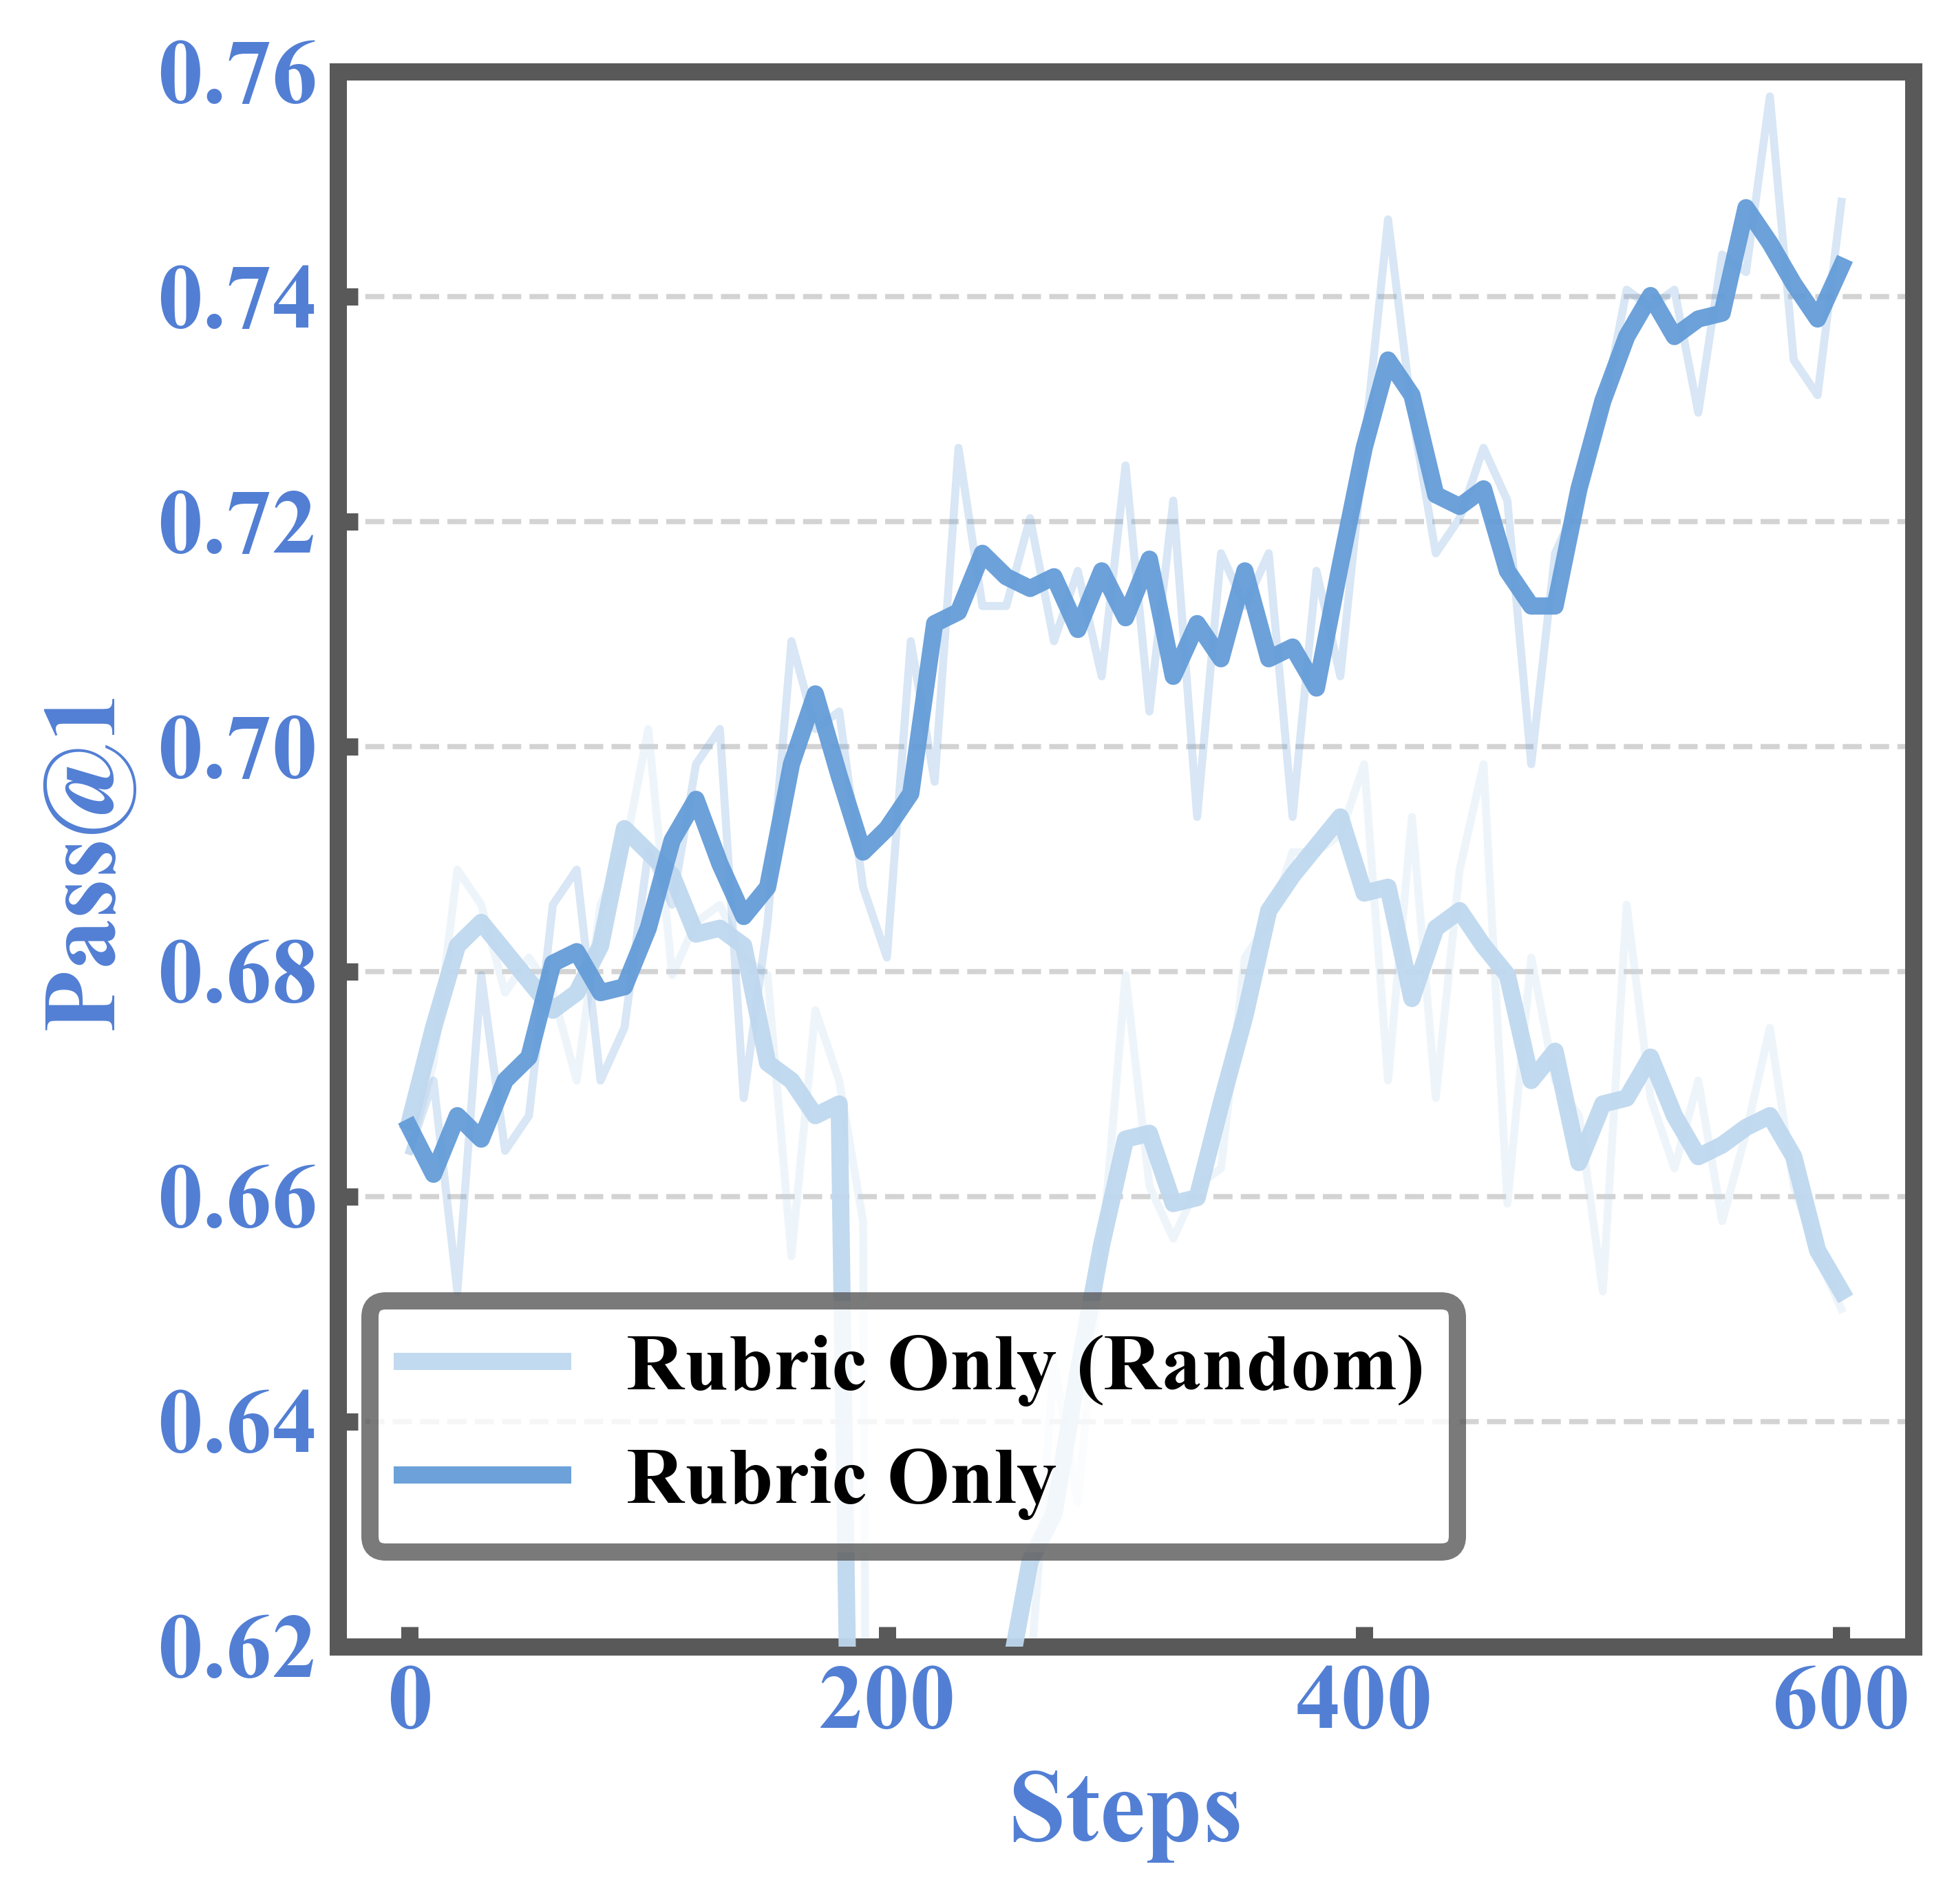
\includegraphics[width=\linewidth]{figures/exp/rubric_only/amc23_rubric_only.png}
    \caption{Accuracy on AMC23.}
    \label{fig:rubric-only-a}
  \end{subfigure}\hfill
  \begin{subfigure}[ht]{0.49\linewidth}
    \centering
    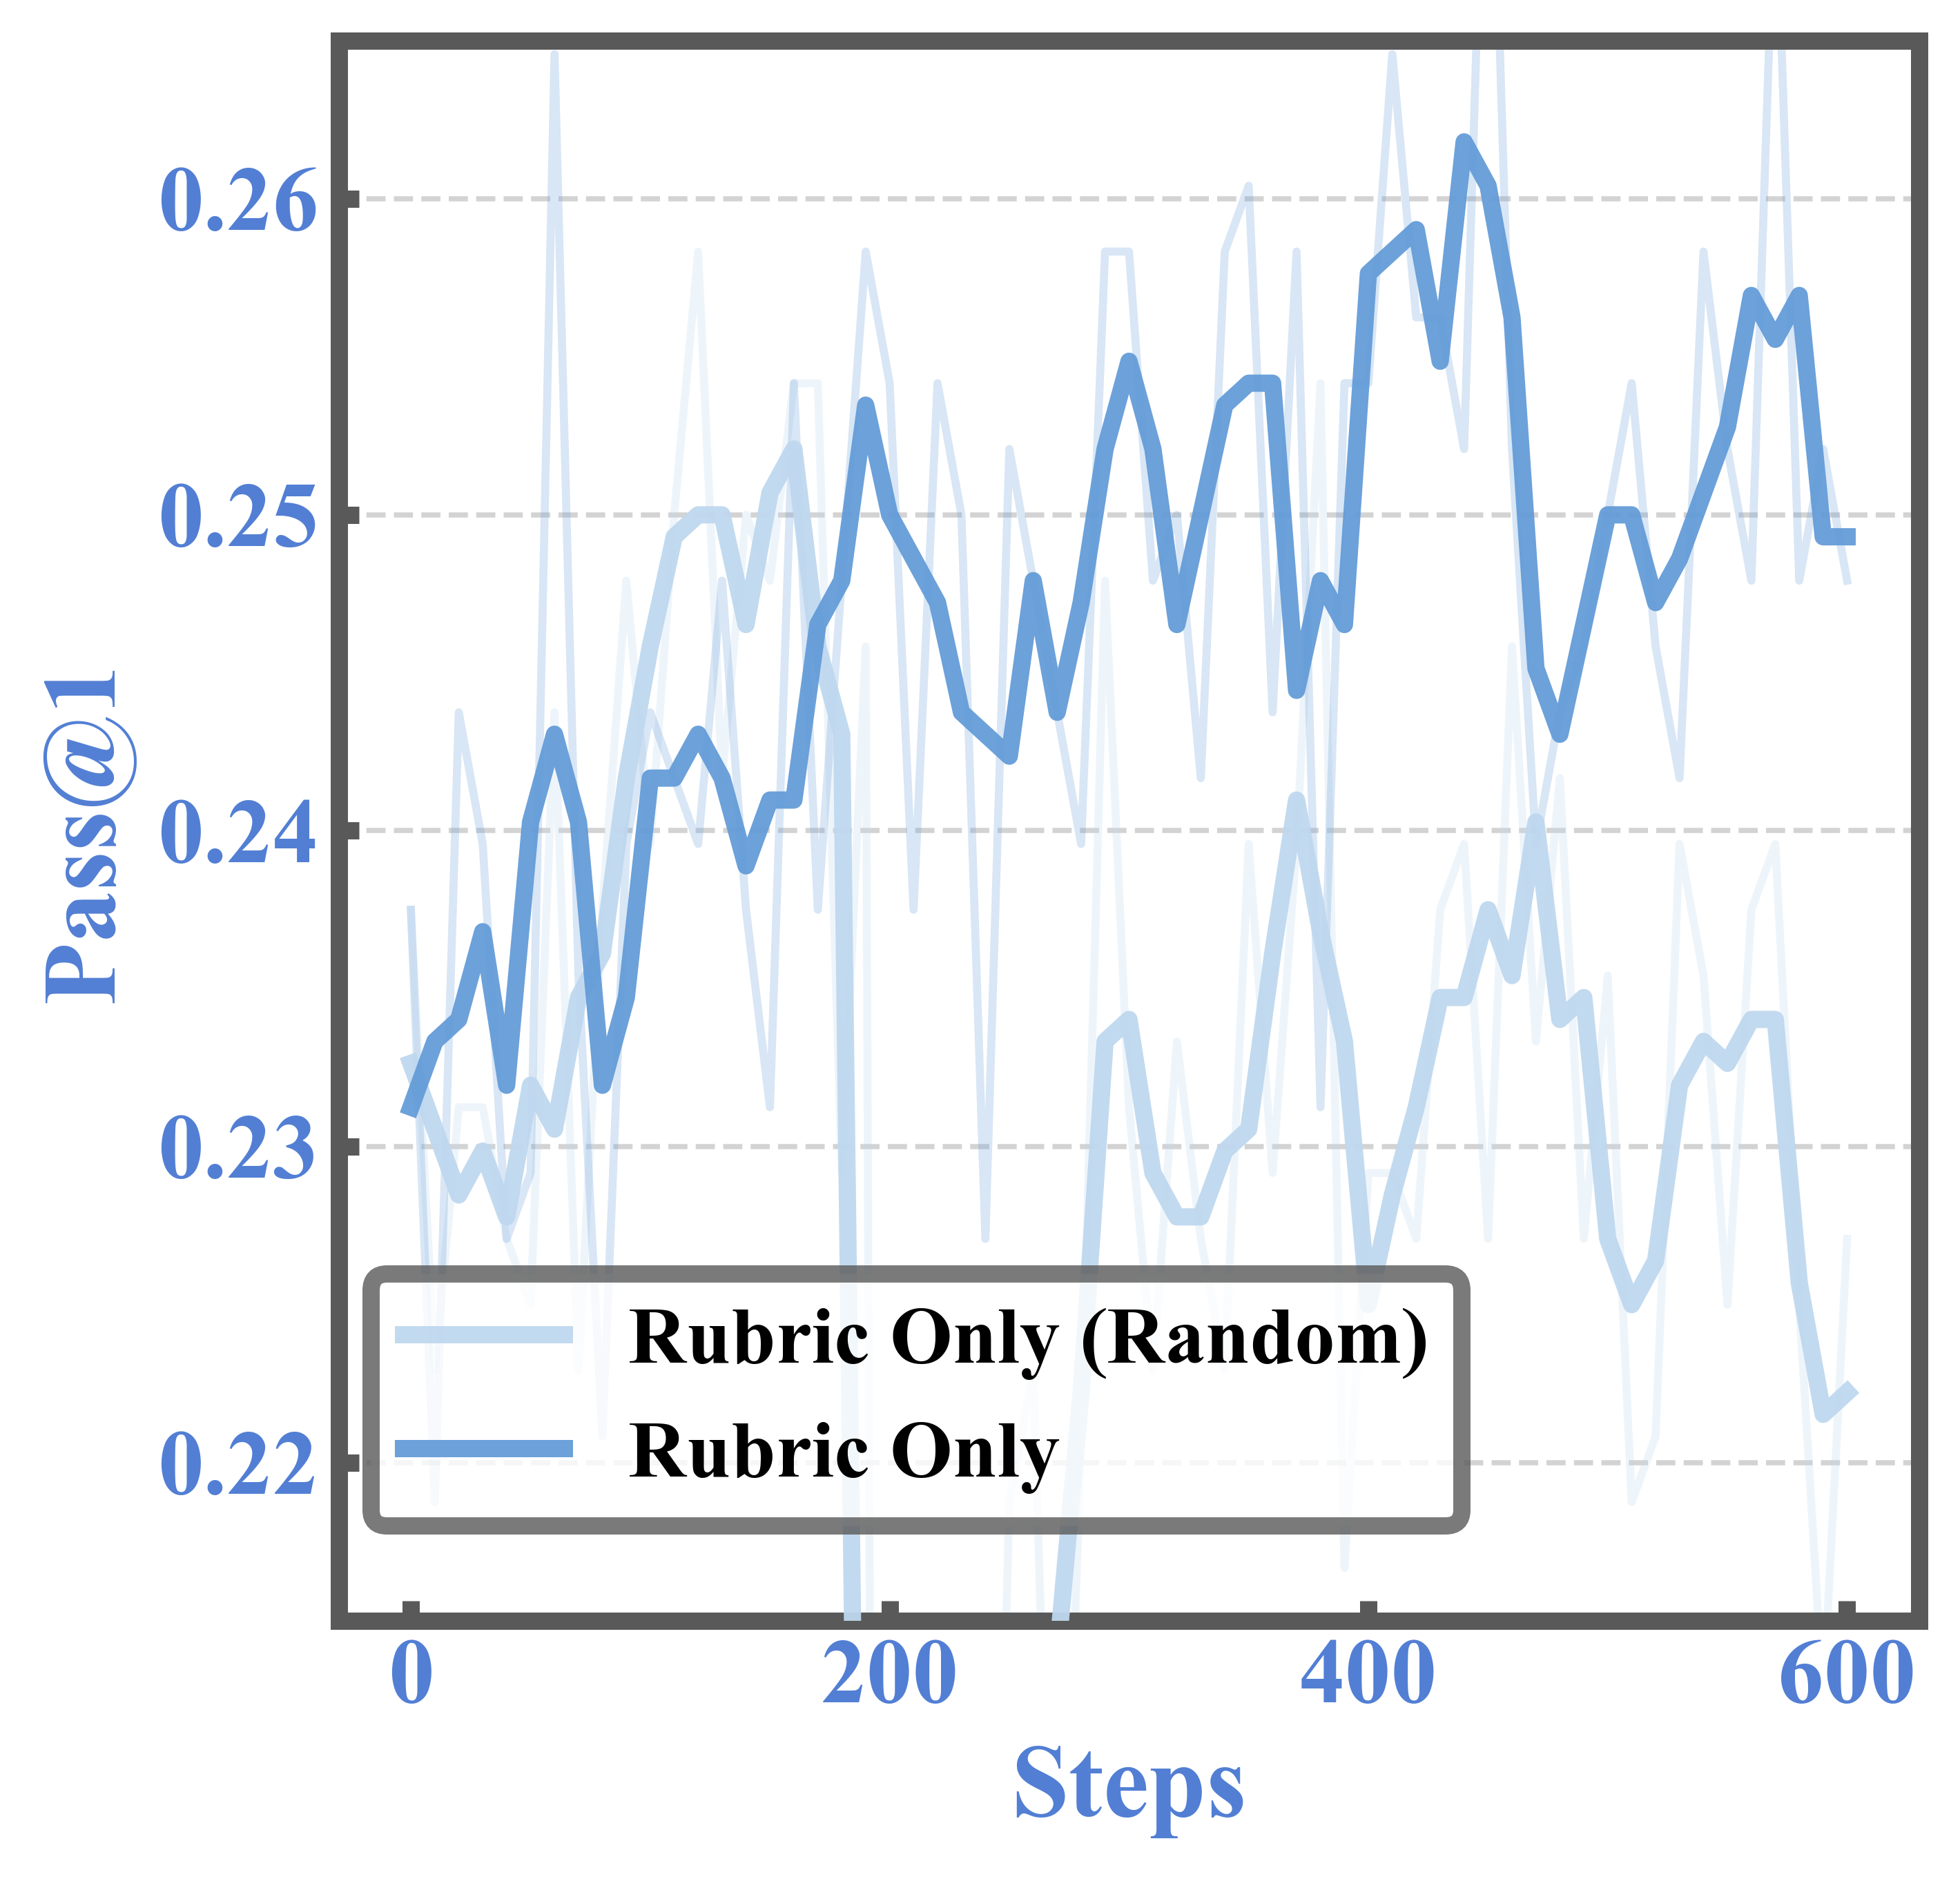
\includegraphics[width=\linewidth]{figures/exp/rubric_only/aime25_rubric_only.png}
    \caption{Accuracy on AIME25.}
    \label{fig:rubric-only-b}
  \end{subfigure}
  \vspace{-10pt}
  \caption{Accuracy dynamics when only rewarding CoTs. Even when rewarding CoTs with self-proposed rubrics without any outcome reward can bring consistent performance gain.}
  \label{fig:rubric-only}
  \vspace{-10pt}
\end{wrapfigure}

A key factor that determines the success of our method lies in whether the self-proposed and self-evolving rubrics can provide meaningful learning signals for RL. 
To verify this, we first conduct a preliminary experiment, considering an outcome-free setting that trains the model by \textbf{only rewarding CoTs based on self-proposed rubrics without any outcome rewards} (\ie $r^{\text{\textcolor{reasoner}{$Rea$}}} =  r_{cot}^{\text{\textcolor{reasoner}{$Rea$}}}$). 
If the model still learns to reason effectively under this setup, it would indicate that self-proposed rubrics can yield meaningful RL signals. 
We report the accuracy dynamics on reasoning tasks during the training in Figure \ref{fig:rubric-only}, where the bold lines are the rolling averaged performance with a window size of 3 and the slim and shallow lines are the original performance. 
We have the following observation:

\textbf{Self-proposed rubrics can provide meaningful CoT rewarding signals for RL training. }
As shown in this figure, by only rewarding CoTs with the self-proposed rubrics (\ie Rubric Only in the figure), the reasoning capability of the LLM shows consistent improvement during training. 
In contrast, when we assign random values between 0 and 1 as rubric rewards (\ie Rubric Only (Random) in the figure), the LLM fails to achieve performance improvements and even exhibits sudden performance drops during training around 200 steps. 
Such results show that the self-proposed and self-evolving rubrics can yield meaningful CoT rewarding signals, which lay an important foundation for our approach RLCER.

\subsection{(RQ2) Effectiveness of RLCER} \label{sec:main-performance}
Based on the reliability of self-proposed rubrics, we further test the effectiveness of combining both $r^{\text{\textcolor{reasoner}{$Rea$}}}_{outcome}$ and $r_{cot}^{\text{\textcolor{reasoner}{$Rea$}}}$ in RLCER. 
We compare RLCER with the vanilla RLVR which only considers the outcome reward, and report the performance comparison in Table \ref{tab:main-table}. 
Here, both RLCER and RLVR start from the SFT checkpoint.
We have the following observations: 


\textbf{RLCER outperforms the outcome-centric RLVR training. }
As shown in Table \ref{tab:main-table}, training with RLCER outperforms the vanilla RLVR across multiple datasets and multiple model sizes on average. 
Even when trained only on math datasets, RLCER also generalizes well on general reasoning tasks (\ie GPQA series.)
Additionally, we observe that the performance gain is more obvious on larger size models (\ie 8B models benefit more from RLCER than 4B models). 
Such phenomena validate the effectiveness of RLCER, which provides a ``free-lunch'' for improving the RL performance, by enhancing it with self-proposed and self-evolving rubrics. 
Case studies about the generated rubrics can be found in Appendix \ref{apdx:case-study}. 



\newcommand{\EMainTableScale}{0.99 }

\begin{table*}[!t]
\centering
\caption{The performance comparison across diverse reasoning benchmarks.}

\makebox[\linewidth][c]{%
  \resizebox{0.92\linewidth}{!}{%
    \begin{tabular}{cl|ccccccc}
    \toprule
    \multicolumn{2}{c|}{\textbf{}} &
    \multicolumn{7}{c}{\textbf{Datasets}} \\
    \textbf{Scale} & \textbf{Method} &
    \textbf{AIME2024} & \textbf{AIME2025} & \textbf{AMC2023} &
    \textbf{GPQA-Diamond} &
    \textbf{SuperGPQA-Eng} & \textbf{SuperGPQA-Med} & \textbf{SuperGPQA-Sci} \\
    \midrule

    % ===================== Scale: 4B =====================
    \multirow{4}{*}{4B}
    & Base
    & 11.25 & 6.46 & 31.09 & 7.77 & 18.50 & 14.25 & 15.44 \\
    & SFT
    & 17.29 & 18.96 & 59.53 & 24.43 & 31.69 & 28.25 & 27.81 \\
    \cmidrule(lr){2-9}
    & + RLVR
    & 29.38 & 30.21 & 79.53 & 44.16 & 39.75 & 28.50 & \textbf{42.88} \\
    & \cellcolor{lightgray}+ RLCER
    & \cellcolor{lightgray}\textbf{29.38}
    & \cellcolor{lightgray}\textbf{30.63}
    & \cellcolor{lightgray}\textbf{81.88}
    & \cellcolor{lightgray}\textbf{44.91}
    & \cellcolor{lightgray}\textbf{40.19}
    & \cellcolor{lightgray}\textbf{31.63}
    & \cellcolor{lightgray}41.81 \\
    \midrule\midrule

    % ===================== Scale: 8B =====================
    \multirow{4}{*}{8B}
    & Base
    & 11.46 & 9.58 & 42.34 & 24.37 & 33.06 & 24.69 & 23.63 \\
    & SFT
    & 22.29 & 23.75 & 66.41 & 31.72 & 36.00 & 33.75 & 35.19 \\
    \cmidrule(lr){2-9}
    & + RLVR
    & 34.79 & 32.50 & 84.53 & 46.56 & 42.94 & \textbf{38.31} & 48.81 \\
    & \cellcolor{lightgray}+ RLCER
    & \cellcolor{lightgray}\textbf{37.50}
    & \cellcolor{lightgray}\textbf{33.33}
    & \cellcolor{lightgray}\textbf{86.41}
    & \cellcolor{lightgray}\textbf{48.77}
    & \cellcolor{lightgray}\textbf{45.00}
    & \cellcolor{lightgray}36.50
    & \cellcolor{lightgray}\textbf{50.25} \\

    \bottomrule
    \end{tabular}
  }%
}

\label{tab:main-table}
\end{table*}

\subsection{(RQ3) Mechanism of Rubrics Self-Evolving} \label{sec:rubrics-self-evolving}


In this section, we study how the rubrics self-evolving affects training within the RLCER framework (\ie the role of the reward $r_{evolving}^{\text{\textcolor{rubricator}{$Rub$}}}$). 
To study this, we conduct an ablation study on the 8B-sized model by abandoning the evolving reward $r_{evolving}^{\text{\textcolor{rubricator}{$Rub$}}}$, and the rubricator is only rewarded with the format reward. 
We report the training dynamics in Figure \ref{fig:ablation-perf} and Figure \ref{fig:ablation-study-wrap} including the averaged performance (\ie averaged accuracy among AIME2024, AIME2025, and AMC2023), the averaged correlation between rubrics satisfaction and final answer correctness (\ie $\mathtt{corr}(\mathbf v_k,\mathbf z)$), and the CoT reward of the reasoner (\ie $r_{cot}^{\text{\textcolor{reasoner}{$Rea$}}}$). 
The performance is reported as the rolling average of 5 scores for a clearer demonstration, where the bold lines report the rolling average scores and the shallow and slim lines report the raw scores.
We have the following observations:


\begin{wrapfigure}{r}{0.52\textwidth}
  \vspace{-10pt}
  \centering

  \begin{subfigure}[t]{0.48\linewidth}
    \centering
    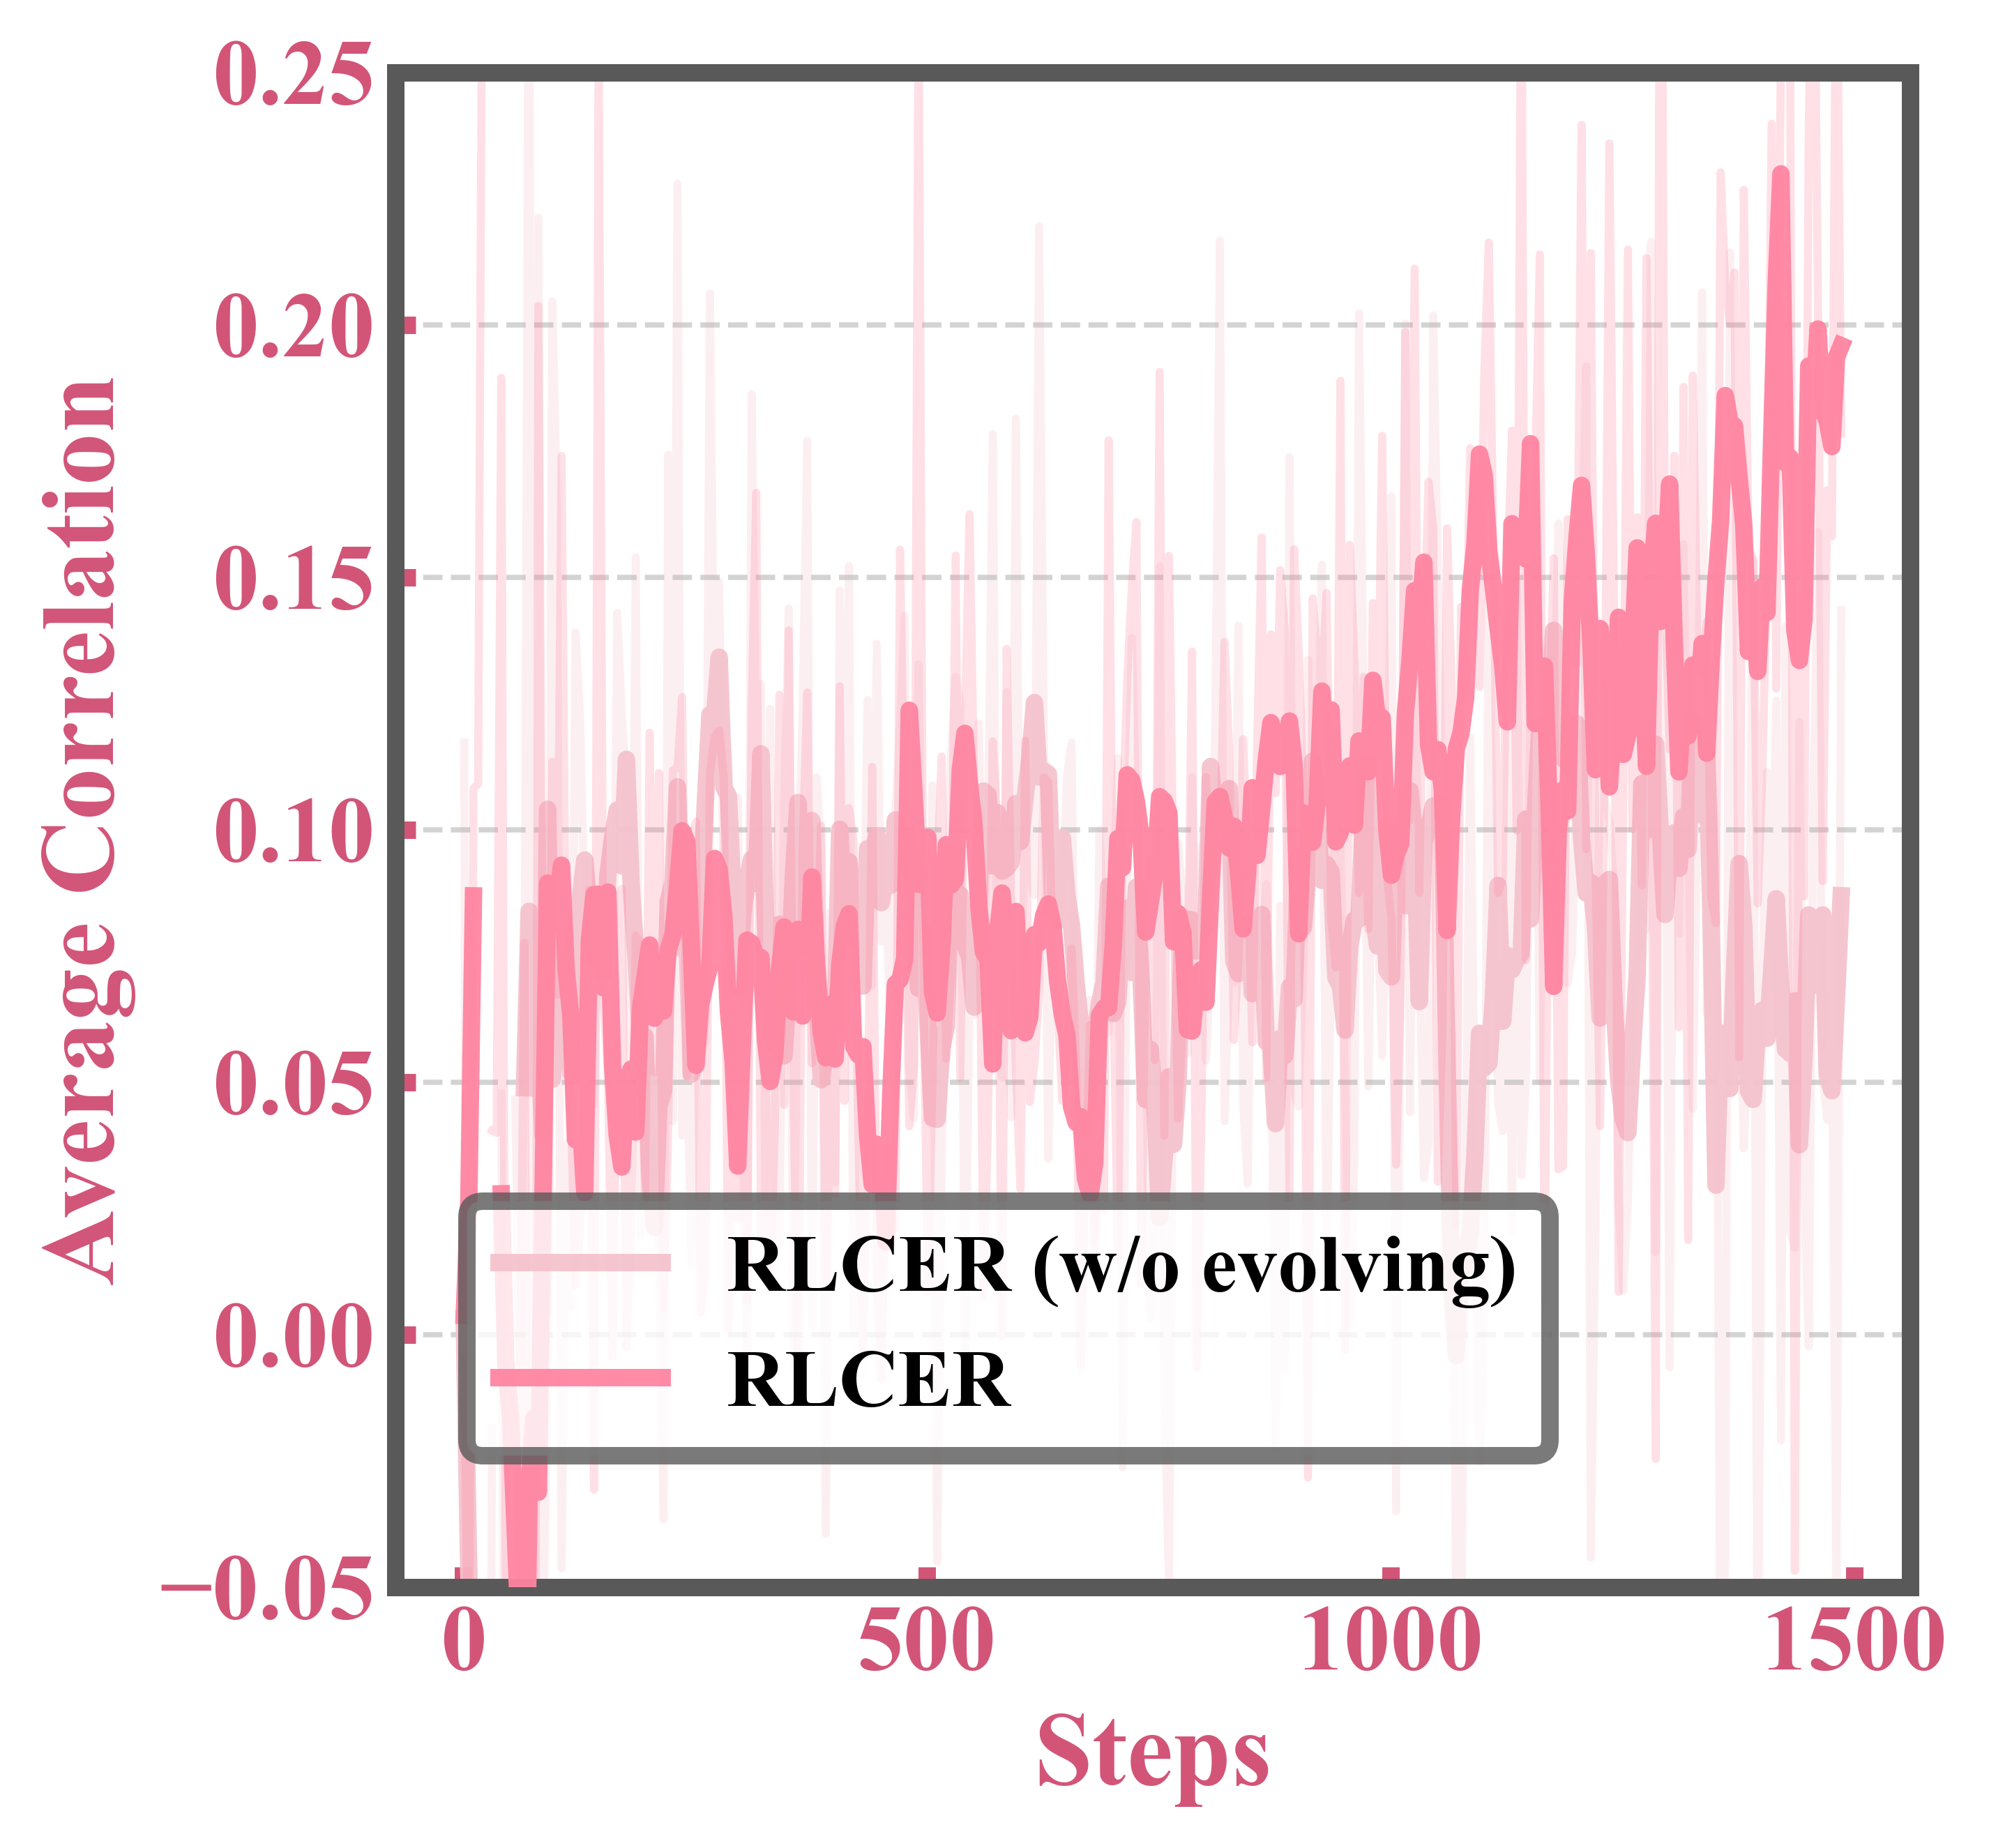
\includegraphics[width=\linewidth]{figures/exp/evolving_ablation/abl_corr.png}
    \subcaption{Correlation dynamics.}
    \label{fig:ablation-a}
  \end{subfigure}\hfill
  \begin{subfigure}[t]{0.463\linewidth}
    \centering
    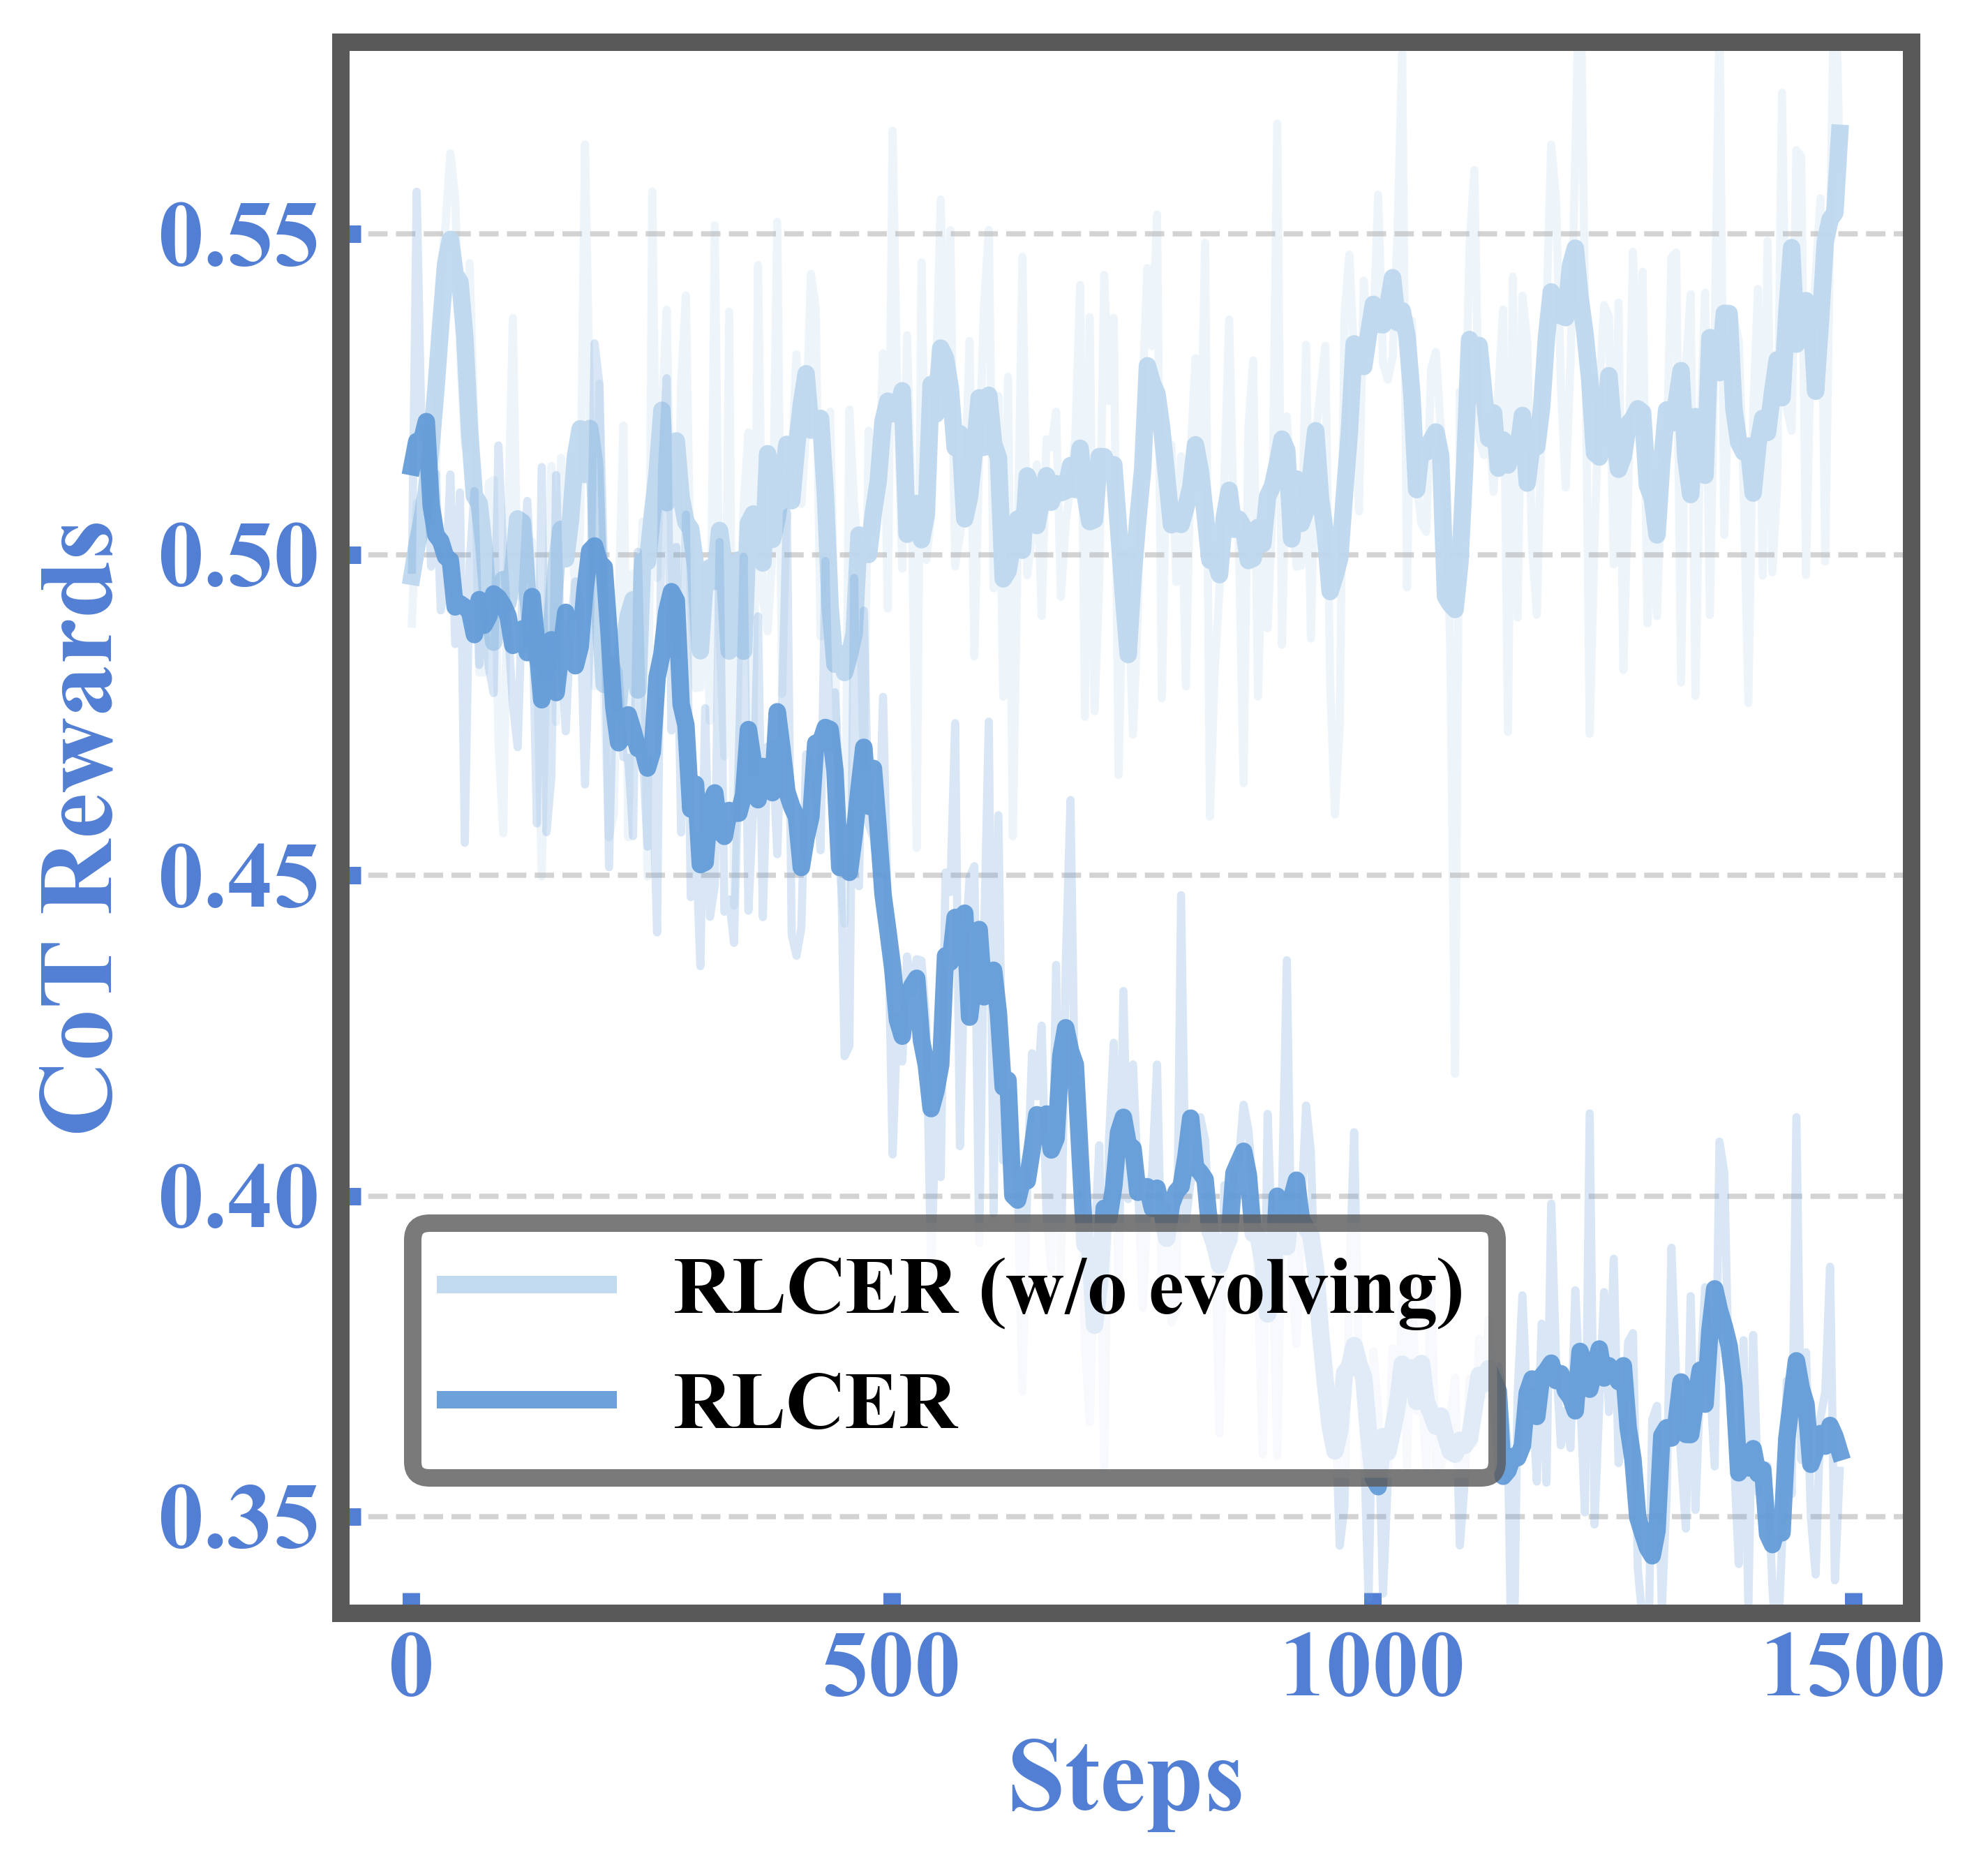
\includegraphics[width=\linewidth]{figures/exp/evolving_ablation/abl_cot_rewards.png}
    \subcaption{$r_{cot}^{\text{\textcolor{reasoner}{$Rea$}}}$ dynamics.}
    \label{fig:ablation-b}
  \end{subfigure}

  \vspace{-8pt}
  \caption{The effect of self-evolving on correlation and CoT-reward dynamics.}
  \label{fig:ablation-study-wrap}
  \vspace{-16pt}
\end{wrapfigure}

\textbf{Self-evolving rubrics enable better performance. }
As shown in Figure \ref{fig:ablation-perf}, by rewarding with $r_{evolving}^{\text{\textcolor{rubricator}{$Rub$}}}$, RLCER exhibits a more stable learning curve and gradually outperforms the ablation version (\ie RLCER (w/o evolving)). 
Additionally, both RLCER and RLCER (w/o evolving) outperform the naive RLVR method as it quickly converges to a sub-optimal performance.
Such phenomena show the effectiveness of self-evolving in enhancing reasoning. 

\textbf{Self-evolving with $r_{evolving}^{\text{\textcolor{rubricator}{$Rub$}}}$ enables more informative rubrics. }
We further analyze whether self-evolving enables the policy model to propose better rubrics.
As shown in Figure \ref{fig:ablation-a}, the averaged correlation between rubric satisfaction and final answer correctness (\ie $\mathtt{corr}(\mathbf v_k,\mathbf z)$) increases along the training process, while the ablation baseline shows an unchanged correlation. 
This indicates that self-evolving enables the policy model to gradually propose more informative rubrics that better align with the final answer correctness. 
Additionally, with such evolved rubrics, it gradually becomes harder to gain the CoT reward $r_{evolving}^{\text{\textcolor{rubricator}{$Rub$}}}$ as the Figure \ref{fig:ablation-b} shows a decreasing trend during the RLCER training. 
While the ablation baseline’s rubrics can be gradually satisfied by $\pi_{\theta}^{\text{\textcolor{reasoner}{$Rea$}}}$ as $r_{evolving}^{\text{\textcolor{rubricator}{$Rub$}}}$ increases. Such results highlight the importance of rubrics self-evolving.

\subsection{(RQ4) Effectiveness of Rubrics as In-prompt Reasoning Hints} \label{sec:rubrics-as-hint}

\begin{wrapfigure}{r}{0.52\textwidth}
  \vspace{-10pt}
  \centering
  % Crop top/bottom to make the square placeholder look wide
  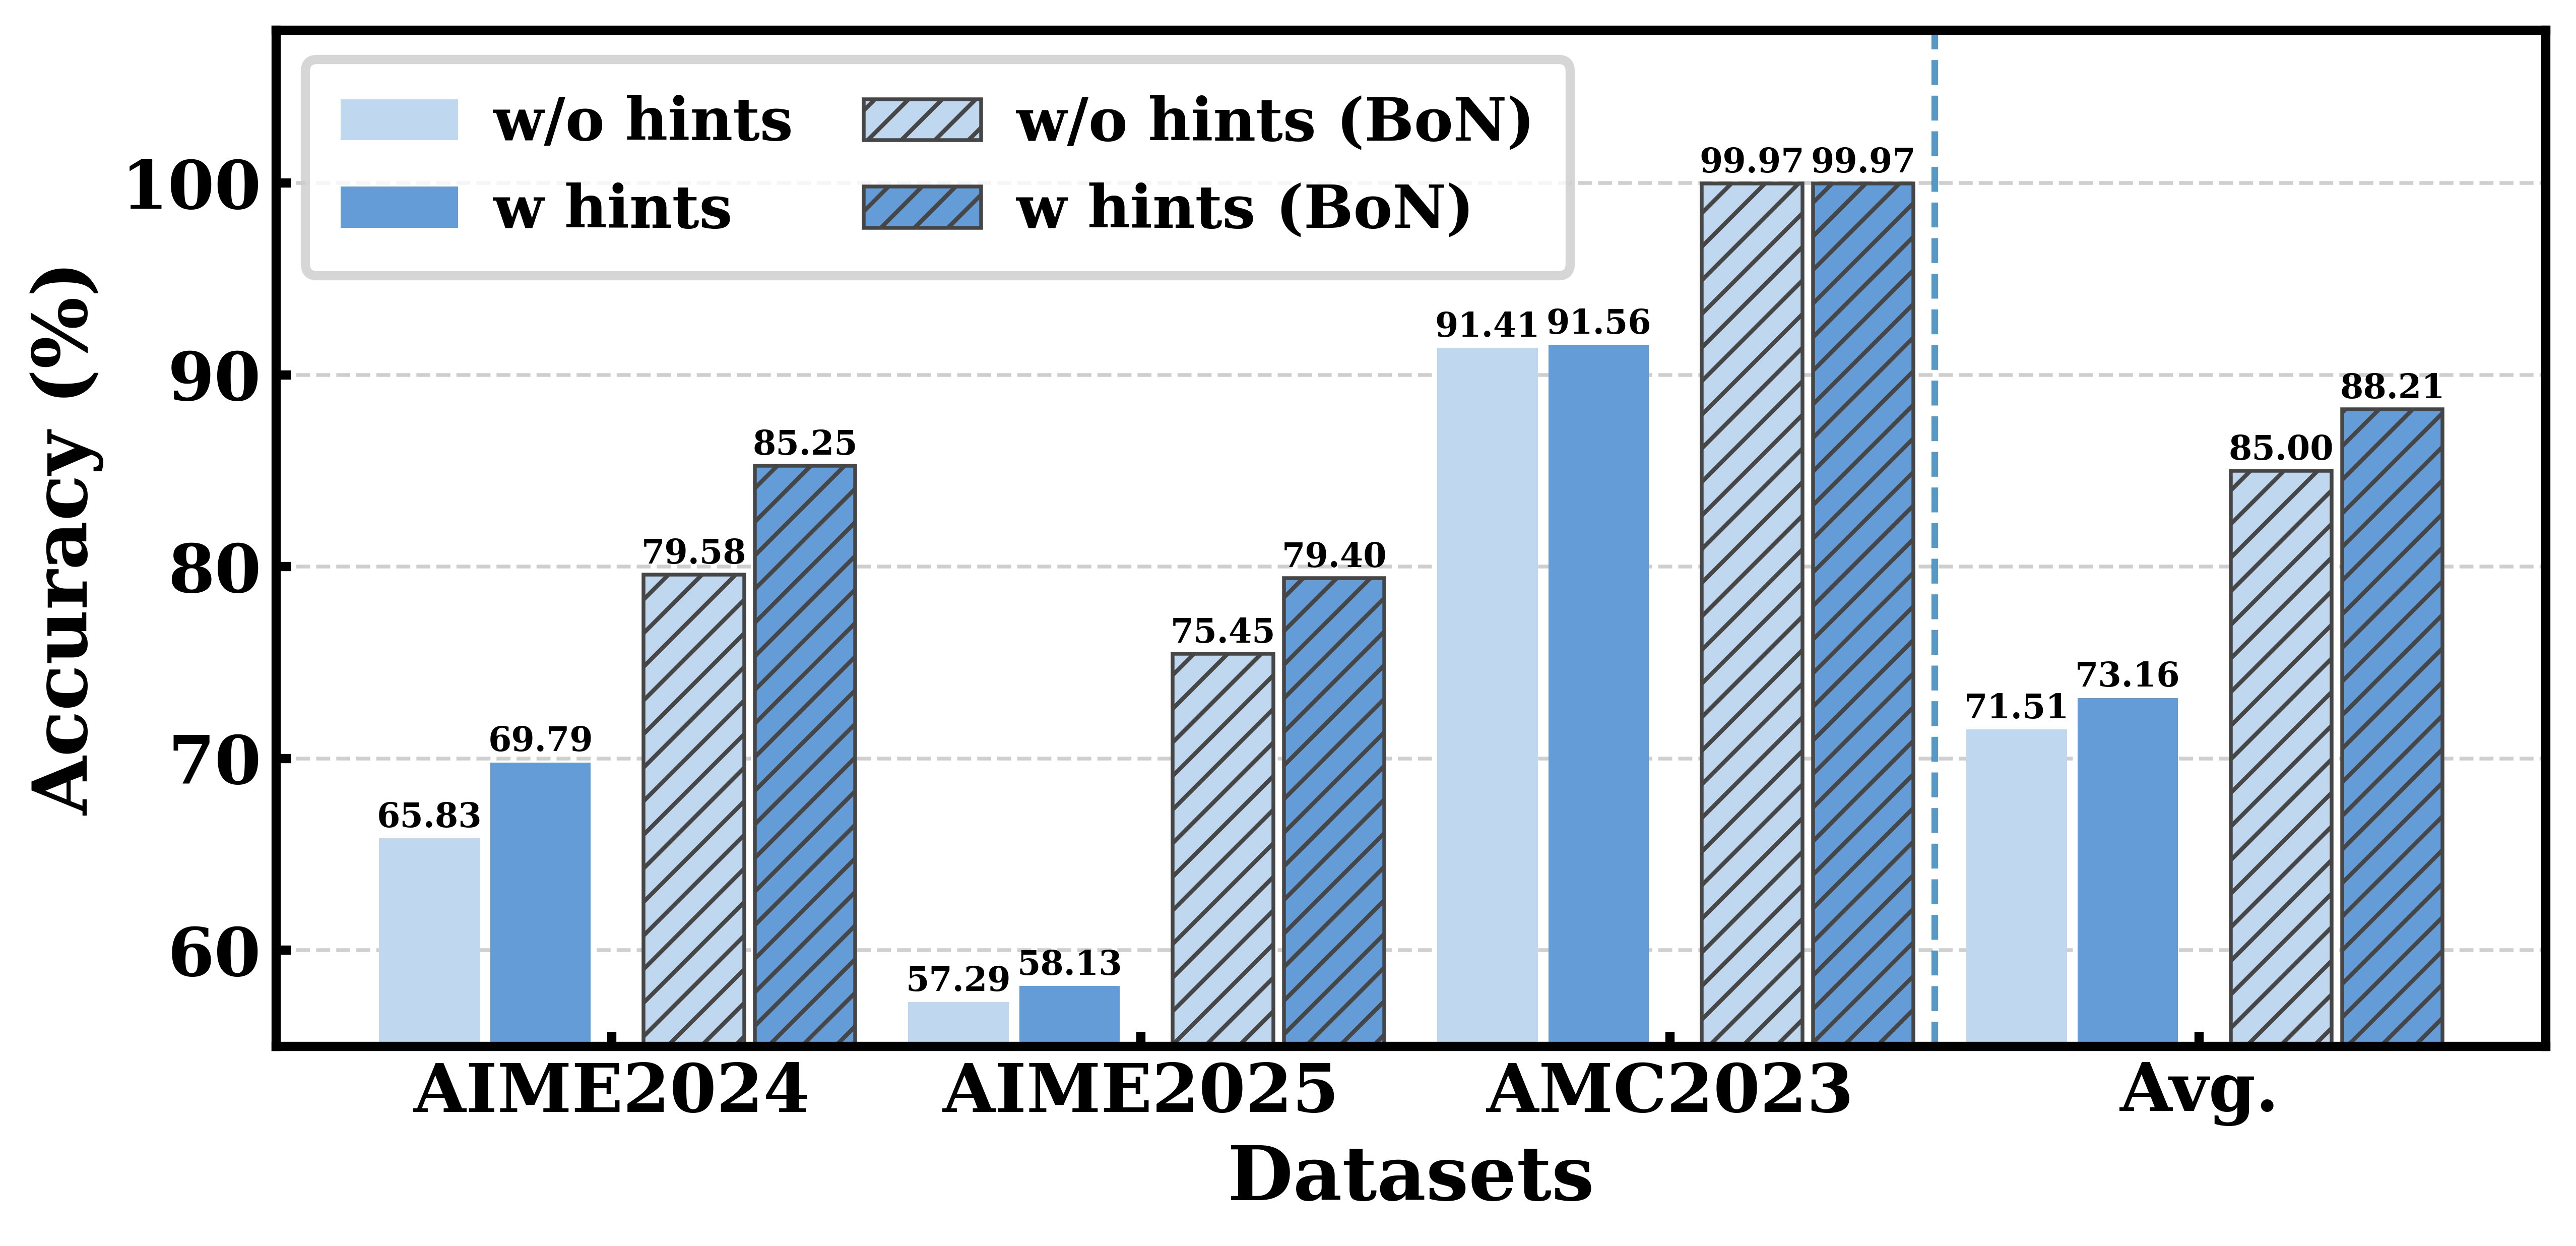
\includegraphics[width=\linewidth]{figures/hints/hints.png}
  \vspace{-20pt}
  \caption{Performance with rubrics as in-prompt hints.}
  \label{fig:rubrics-as-hint}
  \vspace{-10pt}
\end{wrapfigure}

In this section, we attempt to understand how the generated rubrics can guide the model toward better reasoning. 
While we have verified that self-proposed and self-evolved rubrics can generate valid signals for rewarding CoTs, the mechanism through which these rubrics implicitly steer reasoning processes remains elusive, largely because the underlying reward signals are difficult to analyze.
To this end, we explicitly employ these self-proposed rubrics as in-prompt hints, and evaluate the model’s reasoning performance under this setup. 
If incorporating the rubrics into the prompt yields performance improvements, it demonstrates that the rubrics offer valid guidance for the reasoning path. 
We report the performance of Qwen3-8B with a max response length of 20480 in Figure \ref{fig:rubrics-as-hint}. 
As shown in the figure, when using generated rubrics as in-prompt hints, the performance improves, indicating that these rubrics can indeed guide better reasoning. 
Additionally, the performance of BoN (N=16) improved even further on the AIME datasets, indicating that the rubrics introduced as hints may incentivize LLMs to conduct more exploration. 


\renewcommand{\arraystretch}{0.9}

\section{Limitations}
There are still several limitations in this paper.
On the one hand, the introduction of the rubricator role increases the rollout burden and thereby requires more training time.
On the other hand, our method is still quite limited to the RLVR domain, leaving the effectiveness of rewarding with self-proposed rubrics on non-verifiable domains unknown.

\section{Conclusion}
Outcome-centric RLVR improves final-answer accuracy but largely ignores direct supervision for CoTs, risking suboptimal reasoning strategies. 
However, directly rewarding CoT is challenging since reward models are costly to train and brittle under distribution shift and reward hacking. 
To address these issues, we proposed RLCER, which rewards CoTs with self-proposed, self-evolving rubrics without human annotation. 
Experiments showed that RLCER consistently outperforms outcome-only RLVR across datasets and LLM backbones, highlighting that such self-proposed and self-evolving rubrics can provide meaningful CoT supervision signals pushing the upper bound of LLM reasoning. 
Our future work will include exploring the generalization of RLCER to non-verifiable domains. 


\clearpage

\bibliographystyle{plainnat}
\bibliography{main}

\clearpage

\beginappendix
\section{Implementation Details} \label{apdx:impl-details}
We conduct the cold-start training with the LlamaFactory \footnote{https://github.com/hiyouga/LlamaFactory} and all the RL experiments based on the verl \footnote{https://github.com/volcengine/verl} framework. 

\textbf{Cold-start. }
For the cold-start stage, we collect 40k training data from the responses of Doubao-Seed-1.6-thinking \footnote{https://openrouter.ai/bytedance-seed/seed-1.6}, including 20k math reasoning trajectories and 20k rubricator trajectories, which are collected via reject sampling. 
We then perform full-parameter supervised fine-tuning (SFT) on the 40k dataset using Qwen3 prompt template, with a sequence cutoff length of 32768, per-device train batch size = 1, gradient accumulation steps = 1, base learning rate = 2e-5 (cosine scheduler with min lr = 2e-6), weight decay = 0.1, warmup ratio = 0.01 and total training epochs = 5.0. 
For the verifier, we distill a small-sized model Qwen3-4B-Base based on the verification responses from Doubao-Seed-1.6-thinking, using the same SFT recipe as in the cold-start stage.


\begin{table*}[h]
\centering
\begin{tabularx}{0.55\linewidth}{l|c}
  \toprule
\multicolumn{1}{c}{\textbf{Hyperparameter}} \vline & \multicolumn{1}{c}{\textbf{Value}} \\
\midrule
\small
Prompt template                       & Qwen3 \\
Sequence cutoff length                & 32768 \\
Per-device train batch size           & 1 \\
Gradient accumulation steps           & 1 \\
Learning rate (cosine scheduler)      & 2e-5 (min lr = 2e-6) \\
Weight decay                          & 0.1 \\
Warmup ratio                          & 0.01 \\
Epochs                                & 5.0 \\
\bottomrule
\end{tabularx}
\caption{Key training hyperparameters used in the cold-start SFT.}
\label{tab:sft_hyper}
\end{table*}

\clearpage
\textbf{RL training. }
For the RL training, we train all the models with the DAPO-Math-17K data, with prompt max length = 16384, response max length = 12288 (overlong buffer enabled, length = 4096), no KL reward/loss, clip ratio = 0.2, learning rate for actor = 1e-6, learning rate for critic = 1e-5, temperature = 1.0, top\_p = 1.0, train batch size = 32, rollout number $N$ = 8, mini batch size = 64, weight decay=0.1, grad clip=1.0, lr warmup steps=10. 
For all RL training, we fix the max training steps to 1500.
The response length and prompt length are configured in this setting because the outputs generated by the reasoner will serve as the input prompts for the rubricator. Therefore, the max prompt length should be greater than the response length, and the sum of these two values must not exceed 32k tokens. 


\begin{table*}[h]
\centering
\begin{tabularx}{0.4\linewidth}{l|c}
  \toprule
\multicolumn{1}{c}{\textbf{Hyperparameter}} \vline & \multicolumn{1}{c}{\textbf{Value}} \\
\midrule
\small
Algorithm                             & PPO \\
Training dataset                      & DAPO-Math-17K \\
Max prompt length                     & 16384 \\
Max response length                   & 12288 \\
Overlong buffer                       & 4096 \\
KL reward/loss                        & None \\
Clip ratio                            & 0.2 \\
Learning rate (actor)                 & 1e-6 \\
Learning rate (critic)                & 1e-5 \\
Sampling temperature                  & 1.0 \\
Top\_p                                & 1.0 \\
Train batch size                      & 32 \\
Rollout number ($N$)                  & 8 \\
Mini batch size                       & 64 \\
Weight decay                          & 0.1 \\
Gradient clip                         & 1.0 \\
LR warmup steps                       & 10 \\
Max steps                             & 1500 \\
\bottomrule
\end{tabularx}
\caption{Key training hyperparameters used in RL training.}
\label{tab:rl_hyper}
\end{table*}

\clearpage
\section{Prompts} \label{apdx:prompts}
In this section, we report the prompts used as the reasoner $\pi_{\theta}^{\text{\textcolor{reasoner}{$Rea$}}}$ and the rubricator $\pi_{\theta}^{\text{\textcolor{rubricator}{$Rub$}}}$. It is worth mentioning that during our initial attempts to directly prompt Doubao-Seed-1.6-thinking model to generate rubrics based on the question and a reference answer, the model was unable to generate rubrics that are not already presented in the reference. Therefore, we modified the prompt to instruct the model to generate a set of rubrics where the current response score falls below the middle value, and explicitly reinforced this in the format reward. We observed that this practice triggers the model to actively refine rubrics during reasoning to generate meaningful rubrics for room of self-improvement. The 20k rubricator trajectories were then collected using this specific prompt with rejection sampling under such format reward.



\begin{figure}[!ht]
    \centering
    \begin{lrbox}{\DSRPrompt}
    \begin{gptpromptbox}
    \begin{minipage}{0.95\linewidth}
    \raggedright
    % \small\ttfamily
    \scriptsize\ttfamily
\setlength{\baselineskip}{1\baselineskip}
\{question\}

Please reason step by step, and put your final answer within \textbackslash
 boxed\{\}.
\end{minipage}
    \end{gptpromptbox}
    \end{lrbox}
    \usebox{\DSRPrompt}
    \caption{The prompt of the reasoner role.}
    \label{fig:evaluation-prompts}
\end{figure}


\begin{figure}[ht]
    \centering
    \begin{lrbox}{\DSRPrompt}
    \begin{gptpromptbox}
    \begin{minipage}{0.95\linewidth}
    \raggedright
    % \small\ttfamily
    \scriptsize\ttfamily
\setlength{\baselineskip}{1\baselineskip}
You are an expert in educational assessment and rubric design.
Your task is to analyze a given question–answer pair and generate comprehensive evaluation rubrics that can be used to assess response quality for this question. The answer is only a reference answer from the student(not necessarily a good response), so your rubric system should consider the merits already presented in the response, and most importantly, room for further improvements.

\# Input Data

[Question]:
\{question\}

[Response]:
\{response\}


\# Task Instructions

Based on the provided question and answer, generate a comprehensive rubric that's suitable with multiple evaluation criteria. Each criterion should be:\\
1. Specific and Measurable: Clearly define what constitutes meeting or not meeting the criterion\\
2. Binary Evaluable: Can be assessed as true/false by an LLM evaluator\\
3. Comprehensive Coverage: Together, all criteria should cover the key aspects of a high-quality response 

\# Required Rubric Categories

Generate criteria to cover these aspects:
1. Effectiveness of Problem Decomposition \& Planning
Definition: The systematic breakdown of a complex problem into logically ordered, manageable sub-tasks, and the formulation of a strategic roadmap for solving them.
Core Aspects: Identifying key components, establishing step dependencies, sequencing operations, and anticipating challenges before execution.

2. Effectiveness of BackTracking / Self-Validation / Error Handling
Definition: The continuous monitoring of reasoning validity through consistency checks, proactive error detection, and adaptive revision of flawed steps.
Core Aspects: Implementing verification checkpoints (e.g., unit analysis/estimation), diagnosing inconsistencies, recovering from dead ends via path correction (not restarting), and mitigating error propagation.

3. Reasoning Clarity \& Flow
Definition: The coherent structuring and communication of logical progression where each step explicitly follows from prior conclusions and leads to subsequent insights.
Core Aspects: Hierarchical argument organization under clear objective, unambiguous terminology, explicit logical connectors (e.g., "thus," "since," "conversely"), and seamless transitions between ideas.

4. Reasoning Focus \& Efficiency
Definition: The maintenance of strict alignment with problem objectives while optimizing cognitive resources through elimination of redundancies and irrelevant explorations.
Core Aspects: Sustained direction toward core goals, pruning of tangential paths, and avoidance of overthinking/repetition during reasoning.

5. Other Question-Specific Aspects
Definition: The strategic selection and application of domain-relevant methods that align with both problem constraints and solution goals.
Core Aspects: Leveraging context-optimal approaches (e.g., dimensional analysis in physics, elimination methods for multiple-choice), avoiding technique mismatches, and adapting tools to exploit problem structure (e.g., symmetry in geometry).


\# Output Format
Return a JSON object with the following structure:

```json\\
\{\\
  \quad"question\_domain": "math/calculus",\\
  \quad "rubrics": [
    \{
      "category": "Effectiveness of Problem Decomposition \& Planning" 
      "criterion": "XXX",
      "points": 5
    \},
    \{
      "category": "Reasoning Clarity \& Flow" 
      "criterion": "XXX",
      "points": 3
    \},
    \{
      "category": "Reasoning Focus \& Efficiency" 
      "criterion": "XXX",
      "points": 4
    \},
    \{
      "category": "Other Question-Specific Aspects" 
      "criterion": "XXX",
      "points": -3
    \},
    \{
      "category": "Reasoning Focus \& Efficiency" 
      "criterion": "XXX",
      "points": -2
    \}
    // ... additional criteria
  ],\\
  \quad "maximum\_score": a(sum of all positive metrics),\\
  \quad "minimum\_score": b(sum of all negative metrics),\\
  \quad "current\_score": x(must be smaller than (a+b)/2, otherwise revise your rubric system to get better room of improvement) \\
\}\\
```

\# Important Guidelines 
- First output the domain of the question in two levels, then generate 5 - 15 criteria in total, ensuring comprehensive coverage - Points should reflect the relative importance of each criterion (supports positive scores from 1 to 5 for reward criteria, and negative scores from -5 to -1 for penalty criteria). Specifically, a penalty criteria should be a statement that expresses flaw/failure in the reasoning process, while a reward criteria should be a statement that express merits/goal accomplishment in the reasoning process. Some of the final things that your should CHECK BEFORE YOUR FINAL RESPONSE:

\quad - Try to make your rubrics specific to the question, but not so detailed as some of the overly detailed metrics may not apply to all the response(e.g. "fail to apply XXX theorem" would be a acceptable metric, but "fail to reflect after miscalculating using XXX theorem in step25" would be a very bad metric to avoid, since another students response may not apply XXX theorem, nor having step 25). In other words, do not let the reference answer constrain your rubric system!  Again, DO NOT let the reference answer constrain your rubric system!!! To do this, try to propose a set of metrics pretending the reference answer is not there, and reconsider adding some of them. 

\quad - Remember, the answer above is only a reference answer from the student(not necessarily a good response), so your rubric system should consider the merits already presented in the response, and most importantly, room for further improvements. To enforce this, the reference response should have a score strictly below the average of your proposed rubric system. In order to check for this, you need to calculate the maximum\&minimum score from you rubric system, and score the given response at the end of your json. If you found that the rubrics you presented the first time gives a overly-high score, brainstorm more rubrics pretending the reference answer is not there in orderly to find room for improvements and add them to your rubric systems.
- Return only the JSON object without additional commentary.
    
    \end{minipage}
    \end{gptpromptbox}
    \end{lrbox}
    \usebox{\DSRPrompt}
    \caption{The prompt of the rubricator role.}
    \label{fig:evaluation-prompts}
\end{figure}


\begin{figure}[ht]
    \centering
    \begin{lrbox}{\DSRPrompt}
    \begin{gptpromptbox}
    \begin{minipage}{0.95\linewidth}
    \raggedright
    % \small\ttfamily
    \scriptsize\ttfamily
\setlength{\baselineskip}{1\baselineskip}
You are an expert in evaluating student responses to math problems. Your task is to assess a given response based on a set of binary rubrics and compute a final score.

[Task Input]:

- Question: The math problem the student is solving.

- Response: The student's step-by-step solution.

- Rubrics: A list of criteria for evaluation. Each criterion has:

\quad - category: The aspect of reasoning being assessed.
    
\quad - criterion: A binary statement (either a merit to reward or a flaw to penalize).
    
\quad - points: The points assigned (positive for rewards, negative for penalties).

[Task Instruction]:\\
Evaluate each criterion:\\
- For each criterion in the rubrics list (in the given order), determine if the criterion is satisfied by the response.\\
\quad - Output True if the criterion is met (for a reward) or if the flaw is present (for a penalty).\\
\quad - Output False otherwise. \\
- Base your judgement solely on the content of the response and the specific wording of the criterion.\\
- Compute the final score: Sum the points of every criterion that is evaluated as True (this includes both positive and negative points).

[Output Format]\\
Return a JSON object with the following structure:\\
```json\\
\{\\
  \quad "judgement": [boolean, boolean, ...],  // List of True/False for each criterion in the same order as the rubrics\\
  \quad "final\_score": number                  // Sum of points for True judgements\\
\}\\
```

[Important Guidelines]

- Be objective: Do not consider any external knowledge beyond the provided question, response, and rubrics.

- Binary decision: Each criterion must be evaluated as strictly True or False. There are no partial credits.

- Order matters: The judgement list must exactly match the order of the rubrics provided.

- Independent evaluation: Assess each criterion separately. The presence or absence of one flaw/merit does not influence the evaluation of others (unless the criterion explicitly references another).

\quad- Penalty criteria: For a criterion with negative points, True means the flaw is present (so the negative points are added). False means the flaw is absent (so 0 is added for that criterion).

\quad- Reward criteria: For a criterion with positive points, True means the merit is present (so positive points are added). False means the merit is absent (so 0 is added).

Now, proceed to evaluate the following:

Question:
\{question\}

Response:
\{resp\}

Rubrics:
\{rubrics\}

Your final output should contain only the JSON object. Do not include any additional text or explanations.

\end{minipage}
    \end{gptpromptbox}
    \end{lrbox}
    \usebox{\DSRPrompt}
    \caption{The prompt of the verifier.}
    \label{fig:evaluation-prompts}
\end{figure}

\clearpage
\section{Case Study} \label{apdx:case-study}
In this section, we present a case to illustrate how the rubricator proposes meaningful metrics conditioned on the reasoner's response. 
This example shows that the rubricator successfully identifies the key problem(\textit{Employs ad-hoc manual listing for small digit sets instead of systematic permutation formula application, increasing error risk}) that caused miscalculation for $d=0$ and $d=1$ subsets, leading to the final error of 131. It also gives a hint to efficiently solving the problem and reducing reasoning redundancy (\textit{Avoids redundant recounting by categorizing sets with minimum permutation $>$ 2013 upfront, reducing per-set analysis effort}). Therefore, the self-proposed rubrics can effectively guide the model to solve the specific problem, serving as valuable auxiliary reward for the reasoner.

\textbf{Question:}
2013 is the first year since the Middle Ages that consists of four consecutive digits. How many such years are there still to come after 2013 and before 10000?

\textbf{Ground Truth:}
149

\textbf{Prediction:}
131



\textbf{Generated Rubrics:}
\begin{figure}[!ht]
    \centering
    \begin{lrbox}{\DSRPrompt}
    \begin{promptbox}
    \raggedright
    % \small\ttfamily
    \scriptsize\ttfamily
\setlength{\baselineskip}{1\baselineskip}
\{\\
\hspace{2em}"question\_domain":"math/digit-sequence-analysis",\\
\hspace{2em}"rubrics": [\\
\hspace{4em}\{\\
\hspace{6em}"category":"Effectiveness of Problem Decomposition \& Planning",\\
\hspace{6em}"criterion":"Explicitly outlines digit set ranges, leading zero constraints, and year boundary limits before permutation calculations",\\
\hspace{6em}"points":3\\
\hspace{4em}\},\\
\hspace{4em}\{\\
\hspace{6em}"category":"Reasoning Clarity \& Flow",\\
\hspace{6em}"criterion":"Uses hierarchical structuring (e.g., bullet points) for each digit set with explicit permutation counts and exclusion justifications",\\
\hspace{6em}"points":3\\
\hspace{4em}\},\\
\hspace{4em}\{\\
\hspace{6em}"category":"Reasoning Focus \& Efficiency",\\
\hspace{6em}"criterion":"Avoids redundant recounting by categorizing sets with minimum permutation > 2013 upfront, reducing per-set analysis effort",\\
\hspace{6em}"points":3\\
\hspace{4em}\},\\
\hspace{4em}\{\\
\hspace{6em}"category":"Effectiveness of BackTracking, Self-Validation \& Error Handling",\\
\hspace{6em}"criterion":"Fails to implement edge case validation (e.g., overcounting leading-zero permutations) via secondary checklist reviews",\\
\hspace{6em}"points":-4\\
\hspace{4em}\},\\
\hspace{4em}\{\\
\hspace{6em}"category":"Other Question-Specific Aspects",\\
\hspace{6em}"criterion":"Employs ad-hoc manual listing for small digit sets instead of systematic permutation formula application, increasing error risk",\\
\hspace{6em}"points":-2\\
\hspace{4em}\}\\
\hspace{2em}],\\
\hspace{2em}"maximum\_score":9,\\
\hspace{2em}"minimum\_score":-6\\
\}
    \end{promptbox}
    \end{lrbox}
    \usebox{\DSRPrompt}
    \caption{The rubricator's generated rubrics}
    \label{fig:evaluation-prompts}
\end{figure}


\clearpage
\textbf{Reasoner's Response:}

\begin{figure}[!ht]
    \centering
    \begin{lrbox}{\DSRPrompt}
    \begin{promptbox}
    \raggedright
    % \small\ttfamily
    \scriptsize\ttfamily
\setlength{\baselineskip}{1\baselineskip}


Got it, let's try to figure out this problem: we need to find how many years after 2013 and before 10000 have four consecutive digits. First, let's make sure I understand what "four consecutive digits" means in a year (which is a four-digit number, right? Wait, years like 2013 are four-digit, 10000 is five-digit). So a four-digit year with four consecutive digits—wait, does that mean the digits are consecutive in order, like 2013 is 2,0,1,3? Wait no, 2013 isn't consecutive digits. The problem says "2013 is the first year since the Middle Ages that consists of four consecutive digits"—wait, maybe it's digits that are consecutive integers, but not necessarily in order? Wait, wait, let's recheck: "consists of four consecutive digits"—probably, it means the set of digits is four consecutive integers, maybe in any order? Wait, 2013: digits are 2,0,1,3—are those four consecutive? 0,1,2,3 are four consecutive, but 2013 has 0, so 0 is there, then 1,2,3 but missing 2? Wait no, 0,1,2,3 are four consecutive numbers, but 2013 has digits 2,0,1,3—wait maybe I misread: 2013's digits: 2,0,1,3—wait 0,1,2,3 are four consecutive, but is 2013 a permutation of four consecutive digits? Let's list permuted four-digit numbers with digits being four consecutive integers.\\
First, what are four consecutive integers? Let's denote four consecutive digits as d, d+1, d+2, d+3 where d is from 0 to 6 (since d+3 $\leq$ 9, because digits go up to 9). So possible d: 0 (0-3), 1 (1-4), 2 (2-5), 3 (3-6), 4 (4-7), 5 (5-8), 6 (6-9). Wait let's list the sets:\\
d=0: \{0,1,2,3\}\\
d=1: \{1,2,3,4\}\\
d=2: \{2,3,4,5\}\\
d=3: \{3,4,5,6\}\\
d=4: \{4,5,6,7\}\\
d=5: \{5,6,7,8\}\\
d=6: \{6,7,8,9\}\\
These are the possible sets of four consecutive digits (digits are 0-9, so four consecutive can't include 7-10, etc.). Now, a four-digit year can't start with 0, so we need to count permutations of each set that are four-digit numbers (so first digit $\ne$ 0) and are between 2013 and 10000 (so starting from 2014 up to 9999). Wait 2013 is the first since Middle Ages—so we need years after 2013, so starting from 2014.\\
Let's take each set and count valid permutations (four-digit, no leading zero, >2013):\\
\hl{Set \{0,1,2,3\} (d=0): How many four-digit permutations? Total permutations: 4! = 24, minus those starting with 0: 3! = 6, so 18. Now we need permutations >2013. Let's list or calculate: First digit: can be 1,2,3 (since 0 is invalid). If first digit is 1: then the rest are permutations of 0,2,3: 3! = 6 numbers (1023, 1032, 1203, 1230, 1302, 1320). The smallest in this first digit group is 1023, which is less than 2013, so we can ignore all first digit 1 permutations. If first digit is 2: then permutations starting with 2: the remaining digits are 0,1,3. We need permutations >2013. The smallest permutation starting with 2 is 2013, which is the given year. So permutations starting with 2 and >2013: remaining digits 0,1,3—how many are >2013? The smallest is 2013 (which is equal), next would be 2031, 2103, 2130, 2301, 2310. Wait let's count: For first digit 2, second digit: can be 0,1,3 (since 2 is already used). If second digit is 0: then third and fourth digits are permutations of 1,3: 2 numbers (0132 invalid? Wait no, first digit 2, second 0: 2 0 x x—so numbers are 2013, 2031 (since 1 and 3 are digits, so 2013 and 2031). 2013 is equal, so 2031 is >2013. If second digit is 1: then third and fourth digits are permutations of 0,3: numbers are 2103, 2130 (both >2013). If second digit is 3: then third and fourth digits are permutations of 0,1: numbers are 2301, 2310 (both >2013). So for first digit 2: number of permutations >2013: let's count: 2031 (yes), 2103 (yes), 2130 (yes), 2301 (yes), 2310 (yes). That's 5 numbers from set \{0,1,2,3\}.
Set \{1,2,3,4\} (d=1): Four-digit numbers, no leading zero (so first digit 1-4). All permutations are valid since first digit can't be 0. Total permutations: 4! = 24. We need years after 2013. The smallest number in this set is 1234, which is less than 2013, so many numbers here are below 2013. Wait first digit 1: numbers start with 1, so 1xxx, which are all <2000, so ignore. First digit 2: permutations starting with 2: total 6 (since second digit: 3! for remaining 3 digits). These are from 2134 upwards? Wait list them: 2134, 2143, 2314, 2341, 2413, 2431. All these are >2013, right? Yes, since smallest is 2134, which is >2013. So all 6 permutations starting with 2 in this set are valid.}\textbf{==> Employs ad-hoc manual listing for small digit sets instead of systematic permutation formula application, increasing error risk}\\
\hl{Set \{2,3,4,5\} (d=2): First digit can be 2-5 (since no 0 here). So permutations: total 4! =24, minus leading zero? Wait no, no 0, so all 24 are valid four-digit (since first digit 2-5). We need years after 2013. Let's list first digits: 2,3,4,5. First digit 2: permutations starting with 2: 6 numbers (2 \_ \_ \_). The smallest is 2345? Wait no, digits are 2,3,4,5—wait permutations starting with 2: second digit can be 3,4,5 (since 2 is used). So numbers: 2345, 2354, 2435, 2453, 2534, 2543. The smallest in first digit 2 is 2345, which is greater than 2013. So all 6 permutations starting with 2 are valid. First digit 3: permutations starting with 3: 6 numbers (all >2345, so >2013), same for 4 and 5: all 6 each. So total for this set: 6 + 6 + 6 + 6 = 24.\\
Set \{3,4,5,6\} (d=3): Similar to above, digits 3-6, no 0/1. So all four-digit permutations are valid (first digit 3-6). All numbers here are $\geq$ 3456, which is way above 2013, so all 4! =24 permutations are valid.\\
Set \{4,5,6,7\} (d=4): Even higher, 4xxx and above, all permutations valid: 24 numbers.\\
Set \{5,6,7,8\} (d=5): 5xxx and above: 24 numbers.\\
Set \{6,7,8,9\} (d=6): 6xxx and above: 24 numbers.}\textbf{==> Avoids redundant recounting by categorizing sets with minimum permutation > 2013 upfront, reducing per-set analysis effort}\\
Now let's add them up:\\
Set \{0,1,2,3\}: 5\\
Set \{1,2,3,4\}: 6\\
Set \{2,3,4,5\}: 24\\
Set \{3,4,5,6\}: 24\\
Set \{4,5,6,7\}: 24\\
Set \{5,6,7,8\}: 24\\
Set \{6,7,8,9\}: 24\\
Calculations: 5 + 6 = 11; 11 + 24*5 = 11 + 120 = \boxed{\textbf{131}}.\\
    \end{promptbox}
    \end{lrbox}
    \usebox{\DSRPrompt}
    \caption{The reasoner's response}
    \label{fig:evaluation-prompts}
\end{figure}







\end{document}